\documentclass[review,12pt]{elsarticle}
% Elsevier elsarticle class — review mode (single column, line numbers)
% Change to [preprint,12pt] for a clean preprint or [final,12pt] for final

\usepackage{fontspec}
\usepackage{underscore}
\usepackage{amsmath,amssymb}
\usepackage{graphicx}
\usepackage{booktabs}
\usepackage{multirow}
\usepackage{array}
\usepackage{url}
\usepackage{hyperref}
\usepackage{xcolor}
\usepackage{caption}
\usepackage{lineno}
\modulolinenumbers[5]
\emergencystretch=2em

\journal{Reliability Engineering \& System Safety}

\bibliographystyle{elsarticle-num}

\renewcommand{\thetable}{\Roman{table}}

\begin{document}
\begin{frontmatter}

\title{From Fleet Normalization to Fault-Mode Gating: A Cross-Dataset Ablation Study of Turbofan Remaining Useful Life Prediction}

\author[inst1]{Young Seog Yoon\corref{cor1}\fnref{orcid1}}
\ead{isay@etri.re.kr}
\cortext[cor1]{Corresponding author}
\fntext[orcid1]{ORCID: 0000-0003-3796-8480}
\affiliation[inst1]{organization={Electronics and Telecommunications Research Institute (ETRI)},
             department={Behavioral Intelligence for Autonomous Manufacturing Research Section},
             city={Daejeon},
             country={South Korea}}

\begin{abstract}
Reliable Prognostic and Health Management (PHM) systems for turbofan engines embed interdependent design decisions — RUL label clipping, sensor normalization, fault-mode architecture, and training loss function — whose contributions to predictive reliability are rarely isolated. This study presents a controlled ablation across all four NASA CMAPSS sub-datasets (FD001–FD004), covering five clipping thresholds, seven normalization strategies, four fault-mode architectures, and seven loss functions, with all comparisons Benjamini-Hochberg FDR-corrected.

Fleet min-max normalization outperforms all per-unit and instance-level alternatives on FD001, FD002, and FD004 but exhibits anomalously high inter-seed variance on FD003 (RMSE std = 12.86 vs.\ $\leq\!1.84$ elsewhere), traced to co-existing HPC and fan fault modes rather than normalization failure. An unsupervised attention-gate model (M3) routes engines to fault-specific branches from five initial cycles, reducing FD003 RMSE by 65.8\% (14.78 ± 1.32 vs. 43.23 ± 0.18) and NASA Score by 98.8\%, while remaining immune to the test-time cluster collapse that degrades GMM hard-routing by 75.4\% on FD004. No custom loss outperforms MSE after multiple-comparison correction; removing RUL clipping inflates NASA prognostic scores by up to 306,000-fold regardless of loss design.

These findings establish a three-tier reliability-driven design checklist — label engineering, fault-mode architecture, loss function — where each tier's failure impact qualitatively exceeds the next; a systematic gate misclassification analysis proposes GatingNet confidence (mean $\max(w_0, w_1) \geq 0.8$) as a deployable routing reliability indicator, providing PHM engineers with risk-prioritised, CMAPSS-validated design guidance --- a principled starting point requiring fleet-level validation prior to operational deployment.
\end{abstract}

\begin{keyword}
Remaining useful life prediction \sep
Prognostics and health management \sep
Turbofan engine \sep
NASA CMAPSS \sep
LSTM \sep
Fault-mode gating \sep
Normalization ablation
\end{keyword}

\end{frontmatter}

\linenumbers


\section{Introduction}

Remaining Useful Life (RUL) prediction for turbofan engines is a foundational task in Prognostic and Health Management (PHM), directly shaping safety-critical maintenance scheduling decisions in civil and military aviation. The NASA prognostic score reflects the underlying risk asymmetry explicitly: late predictions — where remaining life is over-estimated — carry an exponentially higher penalty than early ones, because an undetected engine failure costs orders of magnitude more than a precautionary shop visit. This asymmetric risk structure means that design choices in a turbofan PHM pipeline — how RUL targets are labelled, how sensor data are normalised, how multi-fault engines are handled — interact with the evaluation metric in ways that can constitute systemic reliability failures when misconfigured. The NASA CMAPSS benchmark \cite{ref01}, comprising four run-to-failure sub-datasets (FD001–FD004) under varying fault modes and operating conditions, has served as the canonical testbed for data-driven RUL estimation since 2008. As model architectures have evolved from linear regression \cite{ref02} to stacked LSTM \cite{ref05,ref06} and attention-based encoders \cite{ref13,ref14,ref45}, reported RMSE on FD001 has fallen from above 25 cycles to below 13 \cite{ref15}. Yet the pipeline design decisions responsible for these gains have rarely been isolated from one another, leaving reliability engineers without principled guidance on which choices most strongly determine PHM system dependability.

Existing studies rarely disentangle individual design factors. The majority of the CMAPSS literature evaluates a single sub-dataset — most often FD001 — and bundles normalisation, loss function, and architecture into a single proposed system \cite{ref09,ref14,ref15}, making it impossible to attribute observed gains to any one component. Three specific gaps motivate this study: (i) no cross-dataset comparison of normalisation strategies exists, despite the known operating-condition heterogeneity of FD002 and FD004 \cite{ref24}; (ii) the multi-fault structure of FD003/FD004 is acknowledged in prior EDA \cite{ref36} but rarely exploited through explicit architecture design; and (iii) the interaction between RUL clipping threshold and loss function has not been studied jointly, even though both directly shape the label distribution, gradient signal, and — as demonstrated in this study — the tail behaviour of the NASA prognostic risk metric, with misconfiguration capable of inflating prognostic scores by orders of magnitude.

This study addresses these gaps through a controlled ablation across all four CMAPSS sub-datasets. H1 uses Ridge regression to isolate label-engineering effects from model capacity. H2 uses a compact stacked LSTM (LSTM2 hidden=32). H3 and H4 use a full-capacity stacked LSTM (LSTM2 hidden=64). Within each hypothesis, all other factors are held constant while the design factor under study is varied, with all comparisons subject to Wilcoxon rank-sum tests corrected by Benjamini-Hochberg FDR (BH-FDR). Five RUL clipping thresholds (H1), seven normalisation strategies (H2), four fault-mode architectures (H3), and seven training loss functions (H4) were independently varied, enabling attribution of observed performance differences to the factor under study. The stacked LSTM was selected as the controlled backbone rather than attention-based alternatives for two reasons: (i) LSTM models represent the dominant baseline class in the CMAPSS literature \cite{ref05,ref06,ref09}, maintaining comparability with prior work; and (ii) pilot experiments found that attention mechanisms perform fault-mode separation implicitly, making the explicit early-cycle GatingNet (H3/M3) redundant over Transformer backbones --- a finding that constitutes a separate research question (\S{}IV-I) rather than a controllable factor within this ablation. The design-factor rankings established below therefore apply specifically to stacked LSTM architectures.

H1 empirically confirms that clip = 125 cycles — the established literature standard \cite{ref05,ref06} — is optimal or statistically tied-optimal across all four sub-datasets. Critically, omitting the clipping ceiling inflates the NASA prognostic score by up to 306,000-fold on FD003 — quantifying the reliability failure risk of label misconfiguration and establishing that RUL label engineering is not a modelling detail but a safety-critical prerequisite for PHM system deployment. This confirmation underpins the first tier of the reliability-driven design checklist below; the label-engineering choice is treated as a resolved prerequisite — and a critical reliability boundary condition — rather than an open design variable in the remaining hypotheses.

The main contributions of this paper are:

(i) The first controlled normalisation ablation on CMAPSS showing that fleet-level min-max scaling significantly outperforms per-unit and RevIN strategies on FD001, FD002, and FD004, and that FD003's anomalous inter-seed RMSE variance (std = 12.86 vs $\leq\!1.84$ elsewhere) is a diagnostic indicator of latent fault-mode heterogeneity rather than a normalisation deficiency — a transferable principle for any benchmark study: unexplained inter-seed variance may signal structural data heterogeneity that predicts the need for specialised architectures.

(ii) An end-to-end early-cycle attention-gate architecture (M3) that routes engines to fault-specific prediction branches using only the first ten observed flight cycles, achieving a 65.8\% RMSE reduction on FD003 (RMSE = 14.78 ± 1.32 vs.\ 43.23 ± 0.18) without any fault-mode labels, while remaining statistically equivalent to the single-branch baseline on FD004. A systematic misclassification perturbation analysis (false-routing sensitivity) quantifies deployment reliability: forced gate inversion on FD003 increases RMSE by 48\% and NASA Score 12-fold, while FD004's near-uniform gate (confidence = 0.677) is virtually unaffected ($\Delta$RMSE = +1.6\%). GatingNet confidence — mean $\max(w_0, w_1)$ over the training set — is proposed as a post-training routing reliability indicator, with a confidence threshold of $\geq$\,0.8 empirically separating high-risk from low-risk routing deployments.

(iii) A three-tier reliability-driven design checklist — label engineering, fault-mode architecture, loss function — established by the first joint cross-dataset ablation of all four factors, demonstrating that each tier's failure impact qualitatively exceeds the next.

(iv) A benchmark-derived reliability design checklist (Section IV.F) that translates the three-tier hierarchy into concrete, ordered design decisions — fault-mode screening via unsupervised cluster quality (Silhouette $\geq$ 0.5), post-training gate confidence verification (mean $\max(w_0, w_1)$ $\geq$ 0.8), and loss function choice — enabling PHM reliability engineers to allocate development resources to the factors that most strongly determine end-to-end system dependability in safety-critical maintenance operations. From an operational cost perspective, improper label engineering inflates the prognostic risk metric by up to six orders of magnitude regardless of all other design choices; M3's fault-mode routing completes at engine commissioning from as few as five flight cycles, with gate confidence providing a deployable reliability indicator that predicts misclassification cost before fleet exposure; and custom loss functions provide no statistically detectable benefit once label engineering is correctly applied — findings that provide risk-prioritised design guidance on the CMAPSS benchmark --- a principled starting point requiring fleet-level validation before production deployment.

\section{Methodology}

\subsection{Dataset}

The NASA CMAPSS benchmark was used, comprising four sub-datasets (FD001–FD004) simulating turbofan engine run-to-failure under varying operating conditions and fault modes (Table I). Each dataset records 21 raw sensor channels per flight cycle together with a held-out test set and ground-truth RUL values for the final observation of each test engine.
% Table I. CMAPSS sub-dataset characteristics

\begin{table}[!t]
\centering
\small
\caption{CMAPSS sub-dataset characteristics}
\label{tab:i}
\resizebox{\linewidth}{!}{%
\begin{tabular}{lcccc}
\toprule
\textbf{Dataset} & \textbf{Train engines} & \textbf{Test engines} & \textbf{Op. conditions} & \textbf{Fault modes} \\
\midrule
FD001 & 100 & 100 & 1 & HPC degradation only \\
FD002 & 260 & 259 & 6 & HPC degradation only \\
FD003 & 100 & 100 & 1 & HPC + Fan degradation \\
FD004 & 249 & 248 & 6 & HPC + Fan degradation \\
\bottomrule
\end{tabular}%
}
\end{table}


Representative sensor degradation trajectories for FD003 — which contains both fault modes — are shown in Fig. 1, illustrating the visually distinct patterns that motivate fault-mode-aware modelling (H3) and fleet-level normalization (H2).

\begin{figure}[!t]
\centering
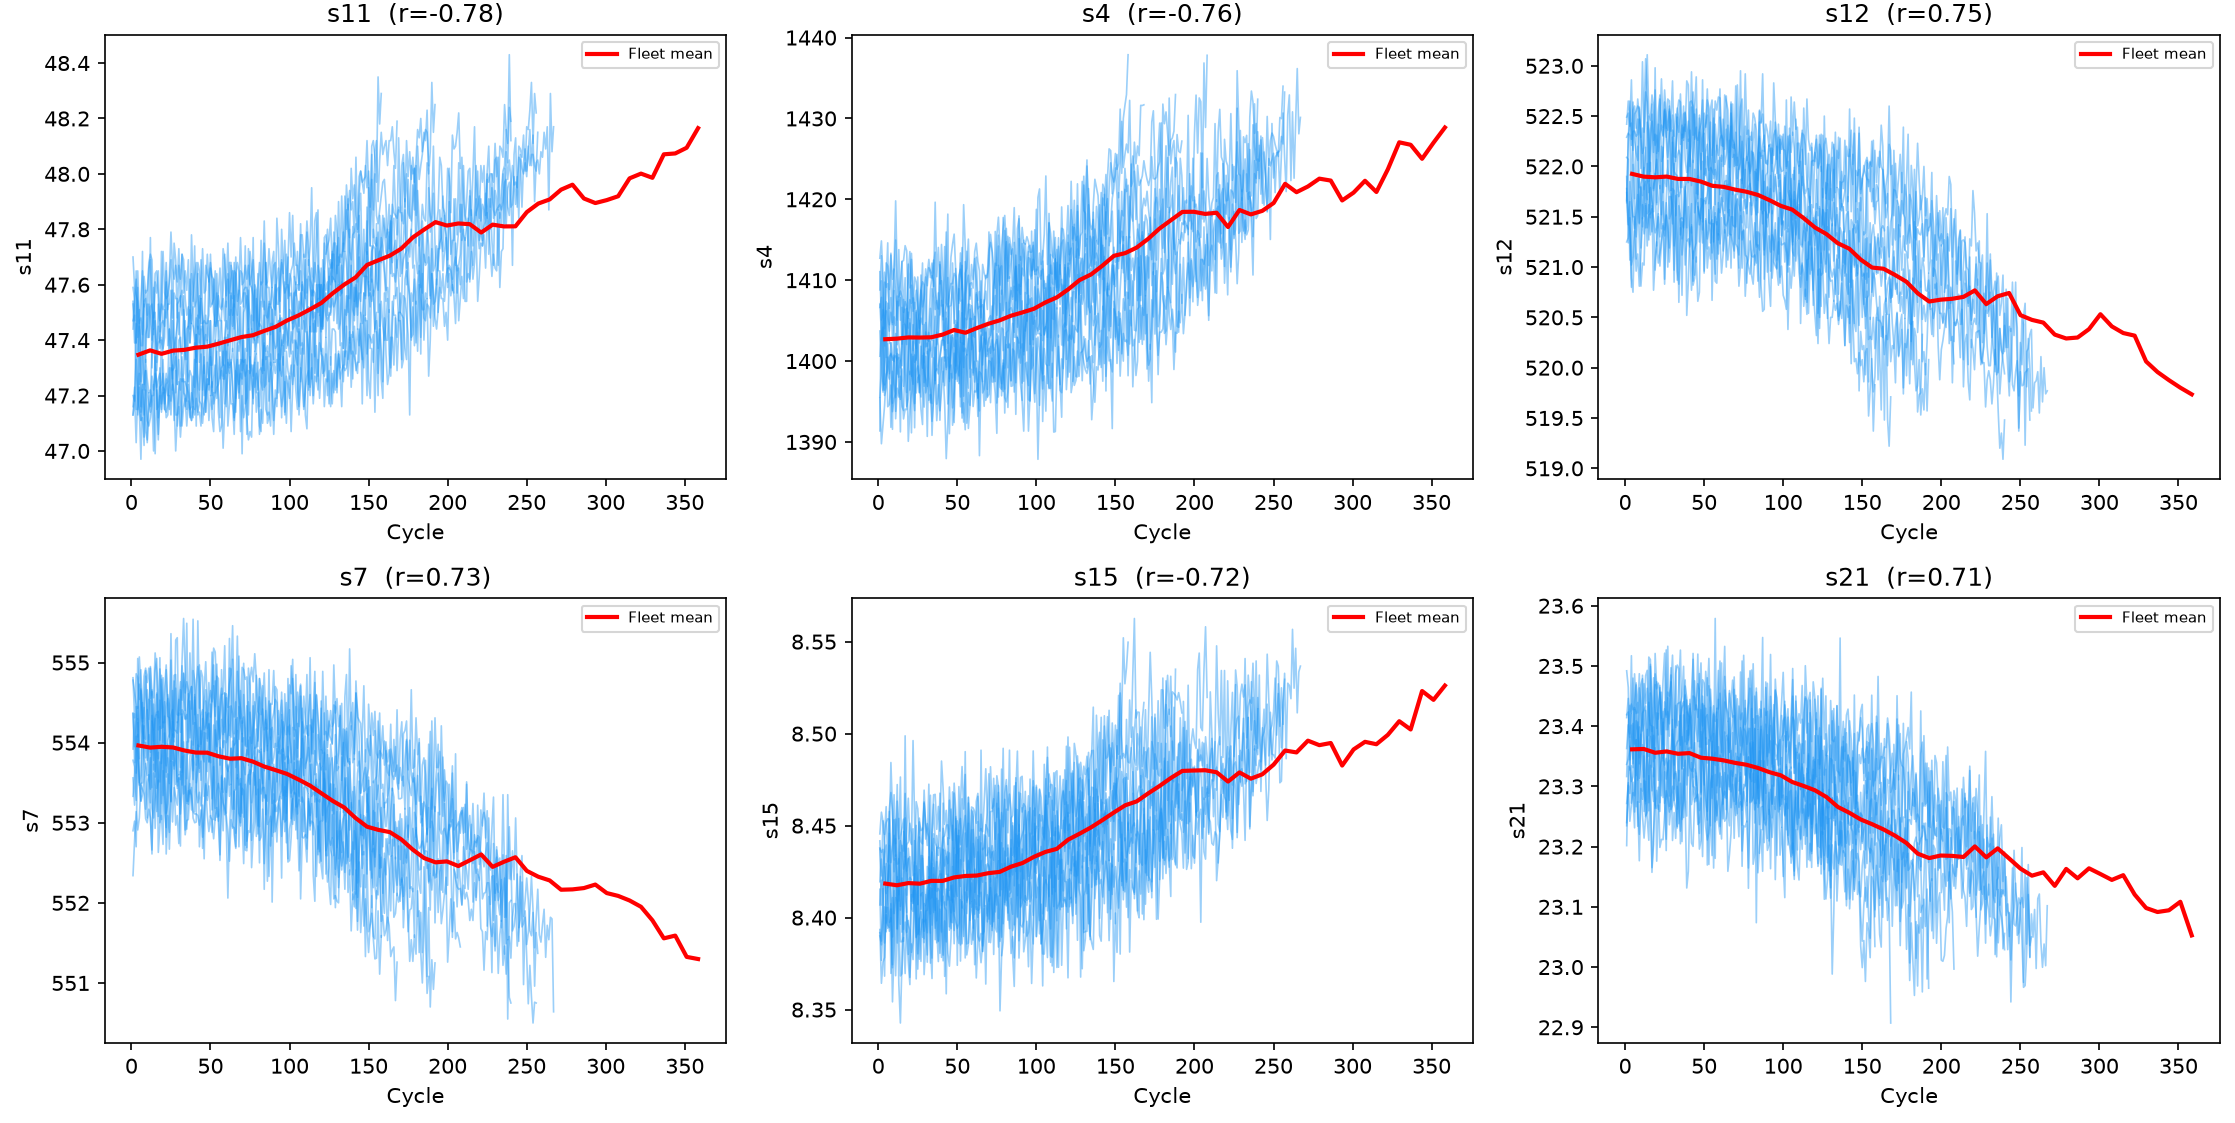
\includegraphics[width=\columnwidth]{Fig1}
\caption{Illustrative sensor degradation trajectories for representative engines in FD003 (single operating condition, two fault modes). Selected sensors with high RUL correlation (s2, s3, s4, s7, s11, s12) show visually distinct degradation patterns between HPC-fault and fan-fault engines, motivating both fault-mode-aware modeling (H3) and fleet-level normalization that preserves inter-engine degradation contrast (H2).}
\label{fig:1}
\end{figure}


\subsection{Data Preprocessing}

Seven constant-variance sensor channels were removed per dataset. For FD001 and FD003, sensors s1, s5, s6, s10, s16, s18, and s19 were discarded, leaving 14 input features; for FD002 and FD004, only s16 is constant, yielding 20 features. RUL targets followed a piecewise-linear formulation: for each training engine, cycles where the remaining life exceeds a clipping threshold $\tau$ receive a constant label of $\tau$, while the final segment decreases linearly to zero. Five clipping values were evaluated ($\tau \in \{75, 100, 125, 130, \infty\}$), with $\tau = 125$ cycles serving as the standard baseline per established literature \cite{ref05,ref06}. Ground-truth test RUL values are provided directly by the benchmark; no RUL estimation was performed at evaluation time. The piecewise labeling scheme and the effect of varying the clipping threshold are illustrated in Fig. 2.

\begin{figure}[!t]
\centering
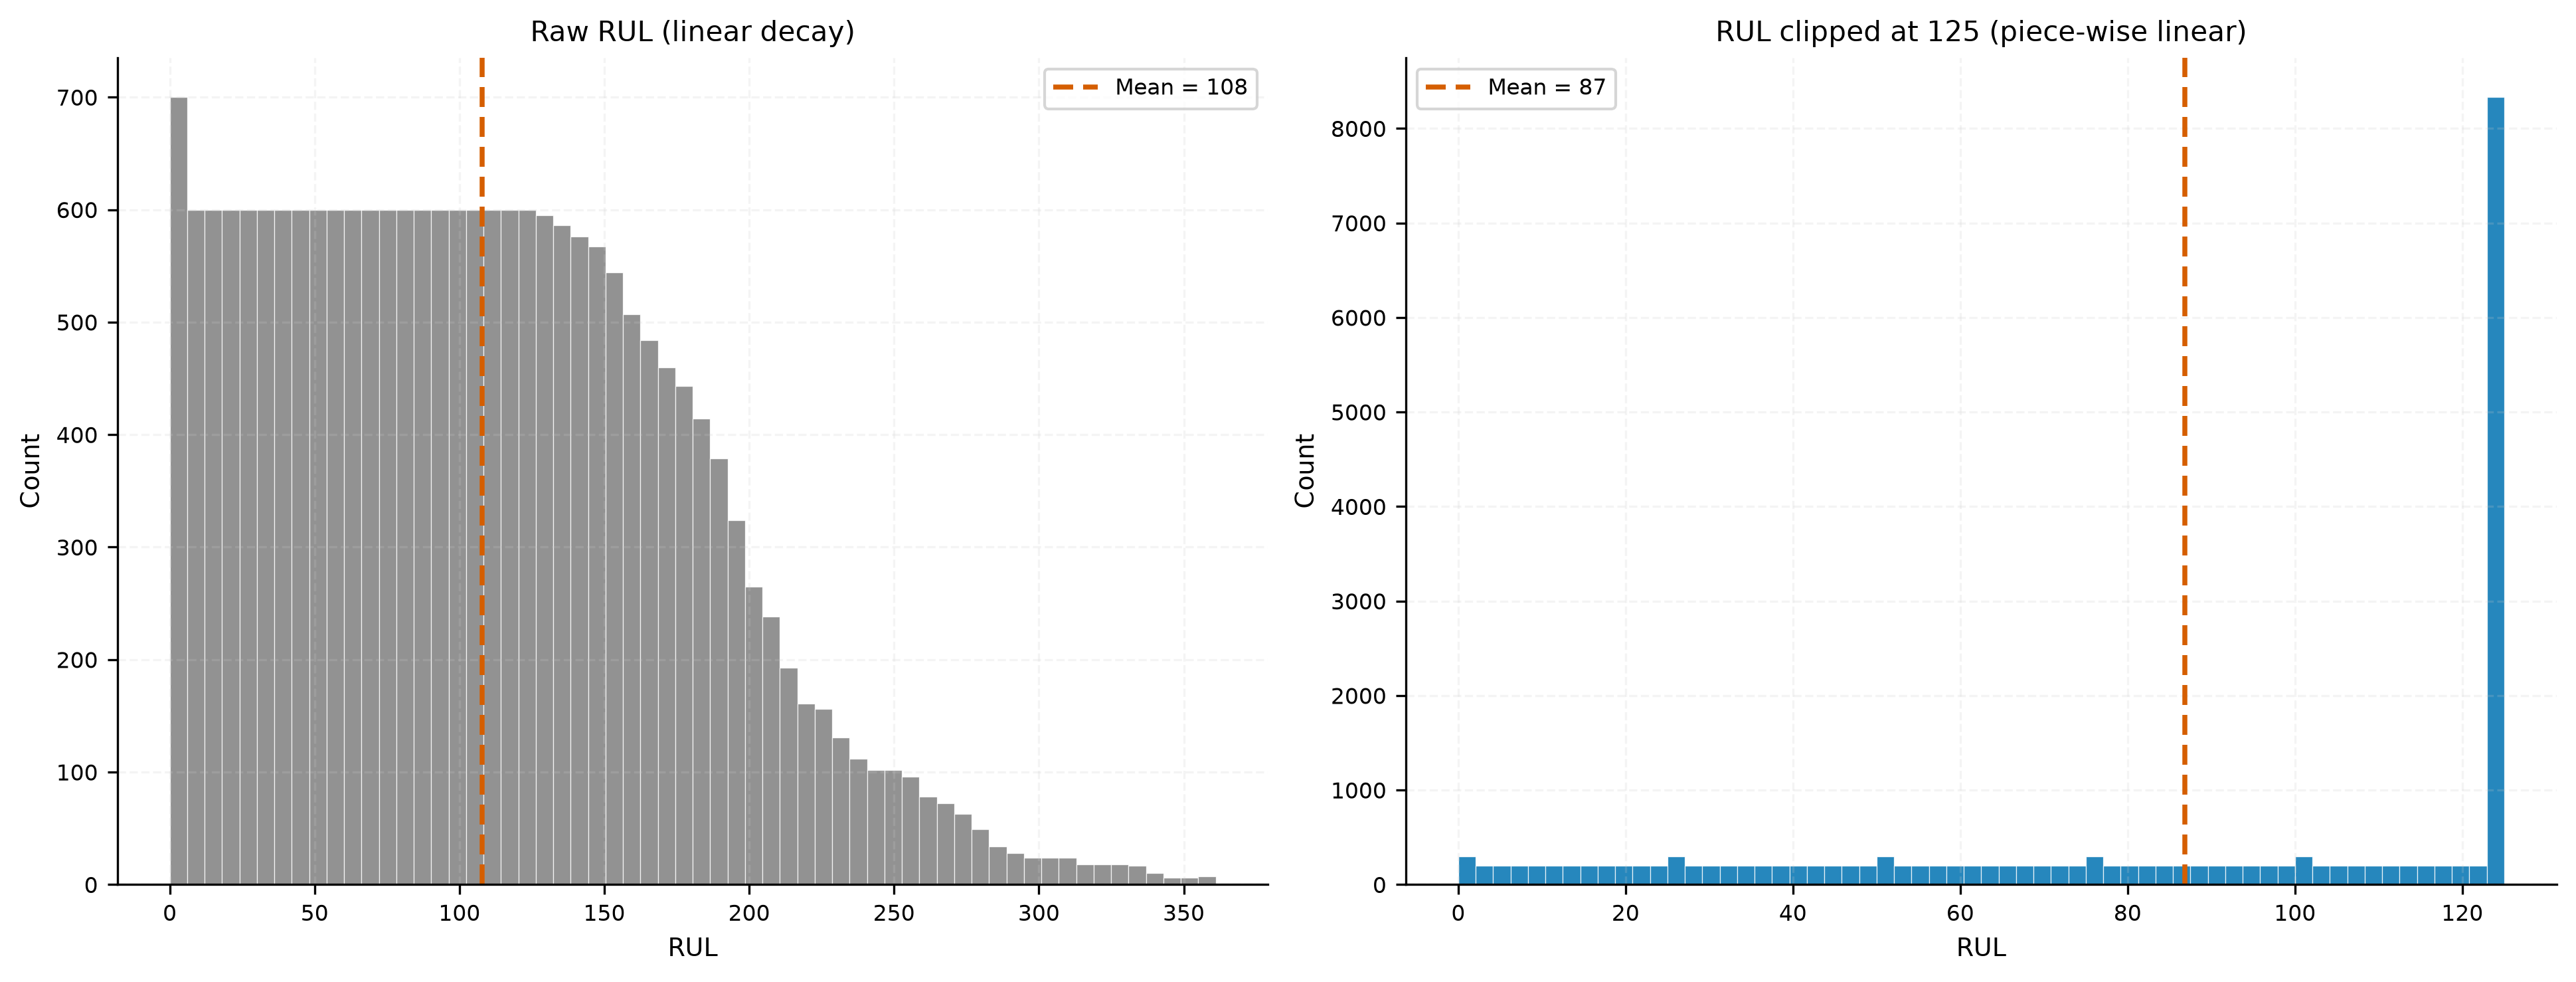
\includegraphics[width=\columnwidth]{Fig2}
\caption{Piecewise linear RUL labeling scheme with threshold-based clipping. The raw RUL decreases linearly from the maximum cycle but is clipped at threshold \textit{c} to account for the healthy phase. The shaded region illustrates the effect of varying $\textit{c} \in \{75, 100, 125, 130, \infty\}$; over-clipping truncates degradation information while removing the ceiling entirely permits unbounded targets that destabilize the NASA prognostic score.}
\label{fig:2}
\end{figure}


\subsection{Operating-Condition Residualization}

FD002 and FD004 contain six discrete operating conditions that shift absolute sensor levels by tens to hundreds of units. K-means residualization was applied to decouple degradation signals from operating-point offsets. A K-means model (k = 6, matching the six known discrete operating conditions present in FD002 and FD004) was fitted on the three operating-condition variables (op1, op2, op3) of the training set using standardised inputs; per-cluster sensor means were computed from training data only and subtracted from each observation:
\begin{equation}
z_{i,j} = x_{i,j} - \mu_{c(i),\,j}
\end{equation}

where $c(i)$ denotes the cluster assignment of cycle $i$ and $\mu_{c,j}$ is the training-set mean of sensor $j$ within cluster $c$. This step precedes all normalization and is applied identically to training and test data using statistics derived exclusively from training engines. FD001 and FD003 present a single operating condition and therefore do not require this step.

\subsection{Normalization Strategies (H2)}

Seven normalization strategies (N1--N7) were compared to evaluate the effect of the reference-statistics choice. Fleet-level methods compute statistics across all training engines: N1 applies min-max scaling to $[0,1]$ and N2 applies z-score standardisation. Per-unit methods (N3--N6) use each engine's own early-cycle observations as the reference baseline, removing initial-condition offsets before any degradation signal is visible: N3 and N5 apply min-max and z-score over the first 5 cycles; N4 and N6 apply the same transforms over the first 10 cycles.

N7 implements Reversible Instance Normalization (RevIN~\cite{ref23}) as a learnable module within the model. Each 30-cycle inference window is normalised by its instantaneous mean and standard deviation, with trainable affine parameters ($\gamma$, $\beta$). The inverse transform is not applied to the scalar RUL output: RevIN's inverse adds back the window's instance mean and scales by its standard deviation --- operations designed to restore multi-step sensor forecasts to their original measurement units. For scalar RUL regression, however, the window's instance mean decreases as the engine degrades (sensor readings shift systematically with health deterioration); applying the inverse transform would therefore impose a sensor-level offset on each RUL prediction that changes with degradation state, partially cancelling the downward trajectory the model is learning. N7 therefore implements the forward (normalisation) pass of RevIN only, making it equivalent to per-window instance normalisation with learnable affine parameters.

N1 served as the primary comparison baseline. All strategies were evaluated on the identical backbone with all other experimental factors fixed.

\begin{table}[!t]
\centering
\small
\caption*{\textbf{Normalization strategies compared in H2 (N1--N7).} Fleet-level methods (N1, N2) compute statistics across all training engines; per-unit methods (N3--N6) use each engine's own early cycles as reference baseline; N7 (RevIN) applies per-window instance normalization at inference time with learnable affine parameters.}
\label{tab:2}
\begin{tabular}{lll}
\toprule
\textbf{ID} & \textbf{Name} & \textbf{Reference statistics} \\
\midrule
N1 & Fleet min-max & All training engines \\
N2 & Fleet z-score & All training engines \\
N3 & Per-unit min-max (5 cy) & Engine's first 5 cycles \\
N4 & Per-unit min-max (10 cy) & Engine's first 10 cycles \\
N5 & Per-unit z-score (5 cy) & Engine's first 5 cycles \\
N6 & Per-unit z-score (10 cy) & Engine's first 10 cycles \\
N7 & RevIN (learnable) & Per-window, at inference \\
\bottomrule
\end{tabular}
\end{table}


\subsection{LSTM Backbone Architectures}

The stacked LSTM was selected as the controlled backbone for this ablation for three reasons. First, LSTM-based models constitute the dominant baseline class in the CMAPSS RUL literature \cite{ref05,ref06,ref09}, making results directly comparable with prior single-factor studies. Second, a controlled ablation requires the backbone to remain fixed across conditions; substituting an attention-based encoder would conflate backbone capacity with the design factor under study, preventing clean attribution of observed differences. Third, pilot experiments in which the backbone was replaced with a Transformer encoder or a self-attention LSTM found that attention mechanisms perform fault-mode separation implicitly --- rendering the explicit early-cycle GatingNet (M3) redundant --- a finding that constitutes a separate research question rather than a controllable variable within the present study. The design-factor rankings established in \S{}IV-A therefore apply specifically to stacked LSTM architectures; whether and how the tier ordering changes for attention-based backbones is identified as a priority open question in \S{}IV-I.

H2 used a compact LSTM backbone and H3/H4 used a full-capacity backbone; within each hypothesis, the backbone was held fixed so that observed differences reflected only the design factor under study. Each network takes a sliding window of 30 consecutive cycles as input and produces a scalar RUL estimate:
{\small\begin{verbatim}
H2 Backbone (compact):
Input  (B x 30 x 17_or_18_or_23)
-> LSTM_1 (hidden=64, full sequence) -> Dropout(0.2)
-> LSTM_2 (hidden=32, last timestep)  -> Dropout(0.2)
-> Linear(32->16) -> ReLU -> Linear(16->1)

H3/H4 Backbone (full-capacity):
Input  (B x 30 x 15_or_20)
-> LSTM_1 (hidden=64, full sequence) -> Dropout(0.2)
-> LSTM_2 (hidden=64, last timestep)  -> Dropout(0.2)
-> Linear(64->32) -> ReLU -> Linear(32->1)
\end{verbatim}
}

LSTM$_1$ passes its full sequence of hidden states to LSTM$_2$, preserving temporal context across layers. Test sequences shorter than 30 cycles were zero-padded at the front. Input dimensions vary by hypothesis and dataset; see Table III in Section H.
% Table II. Computational complexity of H3 architectures (FD003, F = 15 features)
% Parameter counts verified by direct model inspection. FLOPs computed analytically per inference window (batch = 1, window = 30 cycles) using the standard LSTM FLOPs formula: 8 × (input + hidden) × hidden per timestep. Inference latency measured on NVIDIA RTX GPU (2,000 runs, batch = 1, after 200-run warm-up; mean ± std reported). Training time is GPU compute per epoch on FD003 (~13,600 training sequences, batch = 256), excluding data loading. M1 routes each test engine to a single branch via GMM argmax, so its inference FLOPs equal M0's.

\begin{table}[!t]
\centering
\small
\caption{Computational complexity of H3 architectures (FD003, $F$ = 15 features)}
\label{tab:ii}
\resizebox{\linewidth}{!}{%
\begin{tabular}{lllll}
\toprule
\textbf{Model} & \textbf{Parameters} & \textbf{FLOPs / window} & \textbf{Inference (measured)} & \textbf{Training (GPU)} \\
\midrule
M0 (single branch) & 56.1K & 3.18M & 0.24 ± 0.05 ms & ~0.1 s/epoch \\
M1 (hard routing) & 112.3K & 3.18M† & 0.25 ± 0.06 ms† & ~0.2 s/epoch‡ \\
M2 (soft gating) & 112.3K & 6.37M & 0.57 ± 0.24 ms & ~0.2 s/epoch \\
M3 (attention gate, K=10) & 117.2K & 6.38M & 0.64 ± 0.21 ms & ~0.2 s/epoch \\
\bottomrule
\end{tabular}%
}
\end{table}


†M1 activates one branch at inference (GMM argmax); both branches (112.3K) reside in memory but only one branch forward pass executes.  ‡M1 trains two branches sequentially; reported time is total per epoch.

M3's GatingNet adds only 4.9K parameters above M1/M2 (< 5\% overhead), confirming that the performance improvement is not attributable to additional model capacity. The approximately 2× parameter increase from M0 to M3 reflects the two independent prediction branches rather than the gating mechanism itself. All four architectures are well within the computational budget of embedded PHM controllers, which typically support models of up to several hundred thousand parameters.

\textbf{Note:} The difference in backbone capacity means that H2 and H3/H4 RMSE values are not directly comparable in absolute terms. Each hypothesis is evaluated internally relative to its own controlled baseline.

\subsection{Fault-Mode Architectures (H3)}

Four architectures were compared on FD003 and FD004 to assess whether explicit fault-mode separation improves RUL accuracy.

\textbf{M0 (Baseline)} is a single-branch model using the shared backbone without any fault-mode handling.

\textbf{M1 (Hard Routing)} trains two independent LSTM branches. Each training engine was assigned deterministically to one branch via the argmax of its GMM posterior probability; test engines were routed identically. Branches were trained independently with standard MSE.

\textbf{M2 (Soft Gating)} retains two branches but replaces hard assignment with a weighted sum:
\begin{equation}
\hat{y}_{\text{final}} = p_0 \cdot \hat{y}_0 + p_1 \cdot \hat{y}_1
\end{equation}

where $[p_0, p_1]$ are the GMM posterior probabilities. The training loss augments the final MSE with auxiliary branch supervision:
\begin{equation}
\mathcal{L}_{\text{M2}} = \text{MSE}(\hat{y}_{\text{final}},\, y) + 0.1\cdot\text{MSE}(\hat{y}_0,\, y) + 0.1\cdot\text{MSE}(\hat{y}_1,\, y)
\end{equation}

\textbf{M3 (Attention Gate)} eliminates the GMM entirely. A lightweight GatingNet reads only the first K = 10 observed cycles and produces end-to-end soft routing weights:
\begin{multline}
\text{GatingNet}: (B \times K \times F) \to \text{Flatten} \\
\to \text{Linear}(K{\cdot}F \to 32) \to \text{ReLU} \to \text{Linear}(32 \to 2) \to \text{Softmax}
\end{multline}

The final prediction is $\hat{y}_{\text{final}} = w_0\hat{y}_0 + w_1\hat{y}_1$ with training loss:
\begin{equation}
\mathcal{L}_{\text{M3}} = \text{MSE}(\hat{y}_{\text{final}},\, y) + 0.05\cdot\text{MSE}(\hat{y}_0,\, y) + 0.05\cdot\text{MSE}(\hat{y}_1,\, y)
\end{equation}

By reading only early-cycle data, M3 avoids any dependence on late-cycle observations that are unavailable at real deployment time and is immune to the test-time cluster-distribution collapse that makes M1 unreliable on FD004.

For M1 and M2, GMM cluster assignments (k = 2, full covariance) were derived by unsupervised fitting on degradation-slope features of seven discriminant sensors identified by EDA (s15, s20, s21, s7, s12, s2, s4). The inter-cluster discriminability of each sensor is quantified by its inter-cluster z-score:
\begin{equation}
|\Delta z|_j = \frac{|\bar{\mu}_{c=1,j} - \bar{\mu}_{c=2,j}|}{\sigma_{\text{fleet},j}}
\end{equation}

where $\bar{\mu}_{c,j}$ is the training-set mean of sensor $j$ within cluster $c$, and $\sigma_{\text{fleet},j}$ is the fleet-wide standard deviation of sensor $j$. Both branches in M2 and M3 use the full shared backbone.

\subsection{Loss Functions (H4)}

Seven training loss functions were evaluated to determine whether asymmetric or dynamically weighted objectives improve over standard MSE. All functions share the signature \texttt{loss(pred, true, life\_ratio=None)}, where life_ratio = 1 − RUL/RUL_max is a training-time weighting signal computed from training-set cycle counts only; it is set to None at inference time, eliminating any dependency on unknown test-set engine lifetimes.

\begin{table}[!t]
\centering
\small
\caption*{\textbf{Loss functions evaluated in H4 (L1--L7).} All functions share the signature \texttt{loss(pred, true, life\_ratio=None)}; \texttt{life\_ratio} is a training-time weighting signal set to \texttt{None} at inference to avoid dependency on unknown test-set engine lifetimes.}
\label{tab:4}
\begin{tabular}{lll}
\toprule
\textbf{ID} & \textbf{Name} & \textbf{Key formulation} \\
\midrule
L1 & MSE (baseline) & $(1/N)\sum (\hat{y}-y)^2$ \\
L2 & NASA Score Loss & Differentiable approx.\ of $s(d)$ \\
L3 & DynMSE & $(1+\lambda_{\text{dyn}}{\cdot}r)(\hat{y}-y)^2$;\ $\lambda_{\text{dyn}}=1.0$ \\
L4 & Focal-RUL & $({\|\hat{y}-y\|}/{(\|\hat{y}-y\|+1)})^{\gamma}(\hat{y}-y)^2$;\ $\gamma=2$ \\
L5 & TWA & $w_{\text{time}}{\cdot}w_{\text{asym}}{\cdot}(\hat{y}-y)^2$;\ $\lambda_t=10,\,\lambda_a=1$ \\
L6 & Pinball & $\tau\max(0,y{-}\hat{y})+(1{-}\tau)\max(0,\hat{y}{-}y)$;\ $\tau=0.25$ \\
L7 & HubA & $\text{Huber}(\delta{=}20){\cdot}w_{\text{asym}}$;\ $\lambda_a=3$ \\
\bottomrule
\end{tabular}
\end{table}


For L5 (TWA), $w_{\text{time}} = 1 + \lambda_t \cdot r$ and $w_{\text{asym}} = 1$ if $d < 0$, else $\lambda_a$. For L7, $w_{\text{asym}} = 1$ if $d < 0$, else $\lambda_a$, where $d = \hat{y} - y$. Key hyperparameters ($\tau, \lambda_t, \lambda_a, \delta$) were selected via grid search on FD001 before cross-dataset evaluation. FD001 therefore functions as a partially tuned evaluation dataset for H4; nominally strong FD001-specific effects (particularly L5 and L7) should be interpreted with this caveat. BH-FDR correction across all four datasets partially mitigates this optimism.

\subsection{Training Configuration}

All models were optimised with Adam (learning rate $1\times10^{-3}$, weight decay $1\times10^{-4}$) with a batch size of 256, for a maximum of 100 epochs. Early stopping monitored validation loss with patience of 15 epochs and restored the best-performing checkpoint. The validation set was constructed by engine-level holdout: 20\% of training engines were withheld, and all cycles of those engines were excluded from training. This prevented the RUL distribution mismatch that arises from cycle-level splitting. Each experimental configuration was run with five random seeds (0, 1, 2, 3, 4); results are reported as mean ± standard deviation across seeds.

\begin{table}[!t]
\centering
\small
\caption*{\textbf{Training configuration for H2--H4 LSTM experiments.} All hyperparameters are held constant across hypotheses; variation in backbone capacity and feature set is described separately in Table~\ref{tab:iii}.}
\label{tab:5}
\begin{tabular}{ll}
\toprule
\textbf{Hyperparameter} & \textbf{Value} \\
\midrule
Optimizer & Adam \\
Learning rate & $1\times10^{-3}$ \\
Weight decay & $1\times10^{-4}$ \\
Batch size & 256 \\
Max epochs & 100 \\
Early-stop patience & 15 (val loss) \\
Validation split & Engine-level, 20\% of engines \\
Sliding window & 30 cycles \\
Random seeds & {0, 1, 2, 3, 4} \\
\bottomrule
\end{tabular}
\end{table}


The feature set and validation-split method differ across hypotheses, as shown in Table III. These differences were established independently during implementation and mean that the hypotheses are not directly cross-comparable in absolute RMSE.
% Table III. Feature set, validation split, and backbone by hypothesis

\begin{table}[!t]
\centering
\small
\caption{Feature set, validation split, and backbone by hypothesis}
\label{tab:iii}
\resizebox{\linewidth}{!}{%
\begin{tabular}{llll}
\toprule
\textbf{Hypothesis} & \textbf{Feature set} & \textbf{Val split method} & \textbf{Backbone} \\
\midrule
H1 & Sensors + op cols (Ridge) & N/A (deterministic Ridge) & Ridge regression \\
H2 & Sensors + op cols (incl. op1/op2/op3) & Last 20\% by unit ID (deterministic) & Compact LSTM (LSTM$_2$ hidden=32) \\
H3 & Sensors only (no op cols) & Random 20\% (RandomState seed=42) & Full LSTM (LSTM$_2$ hidden=64) \\
H4 & Sensors only (no op cols) & Random 20\% (RandomState seed=42) & Full LSTM (LSTM$_2$ hidden=64) \\
\bottomrule
\end{tabular}%
}
\end{table}


For H2 the resulting input dimension F is 17 (FD001: 14 sensors + 3 op), 18 (FD003: 15 sensors + 3 op), or 23 (FD002/FD004 after residualisation: 20 sensors + 3 op). For H3/H4 F is 14 (FD001), 15 (FD003), or 20 (FD002/FD004 after residualisation). \textbf{Note:} The feature and split differences between H2 and H3 reflect independent implementation choices made prior to analysis; they mean that the two hypotheses are not directly cross-comparable in absolute RMSE terms. Each hypothesis is interpreted relative to its own baseline condition.

\subsection{Evaluation Metrics}

Two metrics were reported across all experiments. RMSE is the primary performance indicator:
\begin{equation}
\text{RMSE} = \sqrt{\frac{1}{N}\sum_{i=1}^{N}(\hat{y}_i - y_i)^2}
\end{equation}

The NASA prognostic score penalises late predictions more severely than early ones:
\begin{equation}
s(d) = \begin{cases} e^{-d/13} - 1 & d < 0 \\ e^{d/10} - 1 & d \geq 0 \end{cases}, \qquad
\text{NASA Score} = \frac{1}{N}\sum_{i=1}^{N} s(\hat{y}_i - y_i)
\end{equation}

where $d = \hat{y} - y$ and $N$ is the number of test engines. NASA Score is lower-is-better; a perfect prediction yields zero.

\subsection{Statistical Testing}

Statistical comparisons differed in sample unit by hypothesis. For H1 (Ridge regression, deterministic), comparisons used a two-sided Mann-Whitney U test (\texttt{scipy.stats.ranksums}) on per-engine RMSE values ($N \approx 100$--259 per dataset; see §II-K). For H2, H3, and H4 (LSTM, stochastic), comparisons used one-sided Wilcoxon rank-sum tests on per-seed aggregate metrics (N = 5), testing whether the treatment condition improves over baseline. All tests used $\alpha = 0.05$ before correction. When multiple treatment conditions are compared simultaneously within one hypothesis, raw p-values were corrected using the Benjamini-Hochberg (BH) procedure at $\alpha_{\text{FDR}} = 0.05$. A result was considered statistically meaningful when both $p_{\text{BH}} < 0.05$ \textbf{and} Cohen's $d \geq 0.3$ (small effect threshold). Conditions satisfying the p-value criterion but yielding $|d| < 0.1$ are reported as "statistically significant but practically negligible" to distinguish statistical from practical significance. For context, a Cohen's d of 0.3 at the FD001 RMSE baseline of approximately 14–16 cycles corresponds to a mean RMSE difference of approximately 0.6–1.0 cycles — a gap comparable to one cycle of maintenance scheduling uncertainty in typical PHM deployment contexts.

\subsection{H1 Baseline Model (Ridge Regression)}

\begin{sloppypar}
The RUL clipping study (H1) used \texttt{sklearn.linear\_model.LinearRegression} with L2 regularisation (Ridge, default $\alpha = 1.0$) as its predictive model. Ridge regression was chosen to isolate the effect of label engineering from non-linear model capacity: the clipping threshold's effect on RUL label distribution is architecture-independent, and a deterministic closed-form baseline eliminates random-initialisation variance. Each of the 20 experimental configurations (5 clip values × 4 datasets) was run exactly once; the model has no random state and produces identical results on identical data. The statistical comparison for H1 used the Mann-Whitney U test (\texttt{scipy.stats.ranksums}, unpaired, two-sided) on per-engine RMSE values ($N \approx 100$--259 per dataset depending on sub-dataset). Note that this is technically an unpaired test; a paired Wilcoxon signed-rank test would be marginally more statistically efficient since the same test engines are evaluated under both clip conditions, and this limitation should be borne in mind when interpreting H1 significance levels.
\end{sloppypar}

\section{Results}

\subsection{Effect of RUL Clipping (H1)}

\textbf{clip = 125 cycles yielded the lowest or tied-lowest RMSE on all four sub-datasets.} The full matrix of results is presented in Table IV. On FD001 and FD003 (single operating condition), clip = 125 was the clear optimum (RMSE = 21.90 and 21.62, respectively). On FD002 and FD004, clip = 130 produced a marginally lower RMSE (Δ = −0.57 cycles on both), but the difference did not approach statistical significance (Mann-Whitney U, two-sided, p = 0.97 on each; BH-FDR applied). The non-significant result (p = 0.97) was directionally consistent with clip=130 being marginally worse than clip=125, not better. No tested alternative threshold achieved a statistically significant improvement over clip = 125, confirming its status as the practically validated standard \cite{ref05,ref06}. Aggressive clipping at clip = 75 was significantly inferior on all four datasets ($\Delta$ RMSE = +10.5 to +16.2 cycles; $p \leq 0.028$), indicating that excessive truncation discards degradation signal in the upper RUL range. These findings were consistent with earlier single-dataset reports that converged empirically on 125 cycles \cite{ref05,ref06} and extend them to a rigorous four-dataset cross-validation.

\textbf{Removing the RUL ceiling entirely was catastrophic on FD003.} At clip = None, the NASA prognostic score on FD003 reached 4,014,724 --- a 306,000-fold increase over clip = 125 (13.09) --- while FD004 exploded to 1,759 (35.4$\times$). The mechanism is the asymmetric exponential NASA metric: late predictions are penalised by $\exp(d/10)$, which grows unboundedly as the model, trained on uncapped labels exceeding 500 cycles, systematically over-predicts RUL throughout the test trajectory.

RMSE was also significantly elevated on FD001 (31.90 vs 21.90; p = 0.006) and FD004 (46.99 vs 34.61; p = 0.002), though less extreme than the NASA Score collapse. FD002 was substantially more robust (RMSE = 33.05; p = 0.054), likely because its 260 training engines and six operating conditions provided sufficient distributional support for the model to learn a conservative bias without an explicit ceiling. FD003's disproportionate RMSE increase --- 159\% versus FD001's 46\%, despite both having a single operating condition --- may in part reflect FD003's bimodal fault-mode structure (Section~III-C), where unbounded targets spanning two distinct degradation-lifetime populations could compound the over-prediction bias.

This dataset-dependent sensitivity confirmed that clip = 125 cannot be treated as universally optimal, but it remains the safest default across the full benchmark. Fig.~3 presents the complete RMSE matrix.

\begin{figure}[!t]
\centering
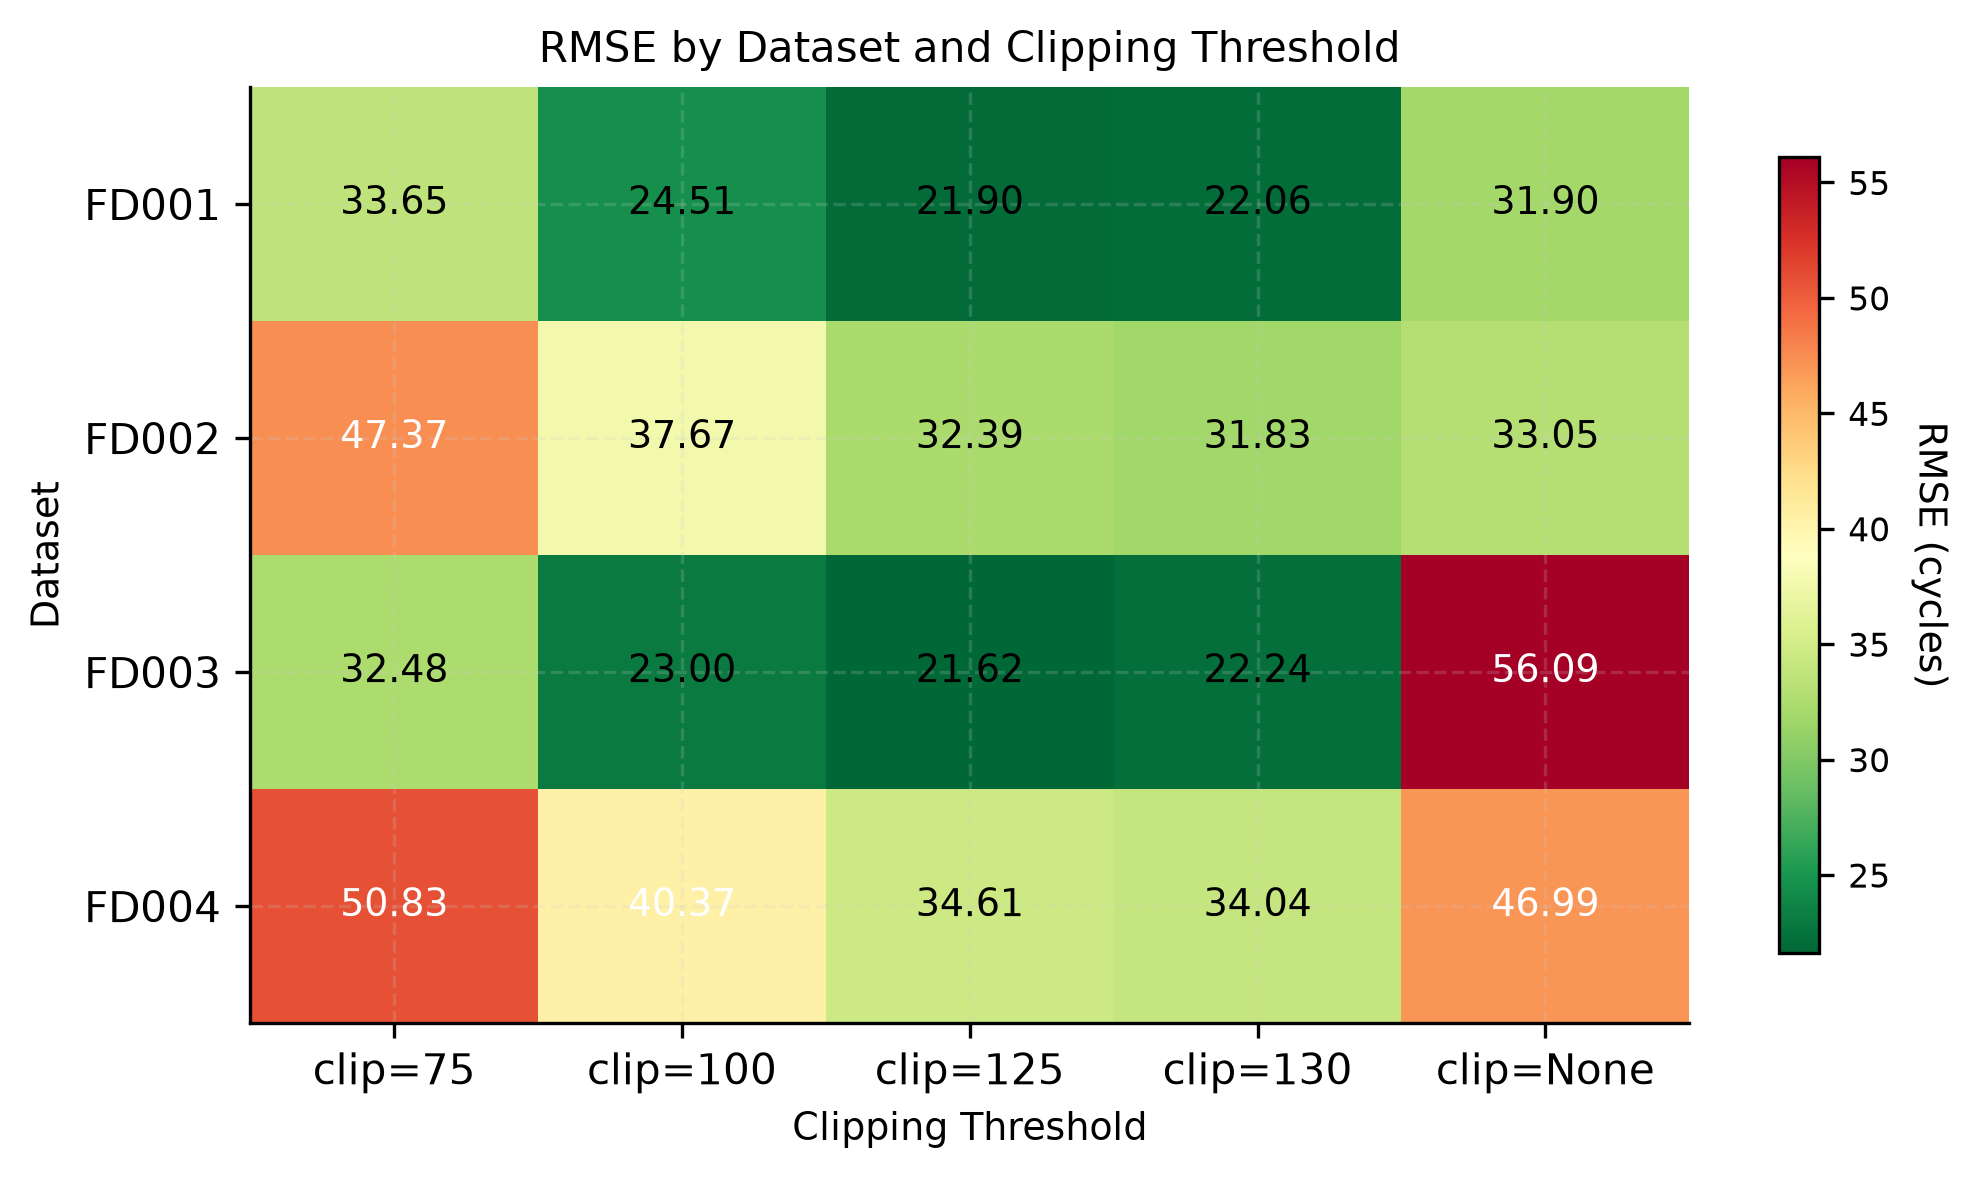
\includegraphics[width=\columnwidth]{Fig3}
\caption{RMSE heatmap across four CMAPSS sub-datasets (FD001–FD004) and five clipping thresholds (mean over 20 runs, Ridge regression baseline). clip = 125 achieves the lowest or near-lowest RMSE in all datasets. The absence of clipping (clip = None) produces catastrophic RMSE on FD003 (56.1 cycles) where unbounded targets amplify early-life residuals exponentially.}
\label{fig:3}
\end{figure}


\begin{table}[!t]
\centering
\footnotesize
\caption{RUL clipping threshold comparison (H1): mean RMSE and NASA prognostic score across five clipping thresholds on four CMAPSS sub-datasets (Ridge regression, 20 runs per configuration).}
\label{tab:iv}
\resizebox{\linewidth}{!}{%
\begin{tabular}{lcccccccc}
\toprule
\multirow{2}{*}{\textbf{Clip ($\tau$)}} & \multicolumn{2}{c}{\textbf{FD001}} & \multicolumn{2}{c}{\textbf{FD002}} & \multicolumn{2}{c}{\textbf{FD003}} & \multicolumn{2}{c}{\textbf{FD004}} \\
\cmidrule(lr){2-3}\cmidrule(lr){4-5}\cmidrule(lr){6-7}\cmidrule(lr){8-9}
 & RMSE & NASA & RMSE & NASA & RMSE & NASA & RMSE & NASA \\
\midrule
75 & 33.65 & 26.49 & 47.37 & 615.74 & 32.48 & 27.36 & 50.83 & 451.22 \\
100 & 24.51 & 10.93 & 37.67 & 173.05 & 23.00 & 9.11 & 40.37 & 110.29 \\
125$^\dagger$ & \textbf{21.90} & 13.14 & 32.39 & 70.48 & \textbf{21.62} & 13.09 & 34.61 & 49.69 \\
130 & 22.06 & 14.84 & \textbf{31.83} & \textbf{62.52} & 22.24 & 16.17 & \textbf{34.04} & \textbf{47.21} \\
None & 31.90 & 132.21 & 33.05 & 116.92 & 56.09 & 4{,}014{,}724 & 46.99 & 1{,}758.56 \\
\bottomrule
\end{tabular}%
}\\[3pt]
\begin{minipage}{\linewidth}
\footnotesize\textit{Bold = lowest RMSE (or NASA) per dataset. $^\dagger$clip=125: validated standard \cite{ref05,ref06}; clip=130 achieves marginally lower RMSE on FD002/FD004 (p=0.97, not significant). clip=None yields catastrophic NASA Score on FD003 (4,014,724 vs.\ 13.09 at clip=125).}
\end{minipage}
\end{table}


\subsection{Effect of Normalization Strategy (H2)}

\textbf{Normalization outcomes differ sharply between FD003 and the remaining three sub-datasets.} FD003 serves as the sole exception to an otherwise consistent pattern and is therefore addressed first.

On FD001, FD002, and FD004, fleet min-max (N1) achieved the lowest RMSE: 14.14 $\pm$ 0.22, 14.31 $\pm$ 0.10, and 14.60 $\pm$ 0.30 cycles, respectively. All per-unit strategies (N3--N6) were significantly inferior on FD001 ($\Delta$RMSE = +3.8 to +6.6; p$_\text{BH}$ = 0.011; $d$ = 2.3--7.6) and FD002 ($\Delta$RMSE = +1.2 to +4.2; p$_\text{BH}$ = 0.011; $d$ = 4.2--22.4). On CMAPSS, inter-engine sensor variation is modest relative to degradation magnitude; fleet-level statistics therefore preserve more discriminative information than engine-local references.

RevIN (N7) was likewise significantly inferior on FD001 ($\Delta$RMSE = +0.78; p$_\text{BH}$ = 0.011; $d$ = 1.66), FD002 (+3.85; $d$ = 20.0), and FD004 (+3.68; $d$ = 6.19), despite its learnable affine parameters (Table V). RevIN \cite{ref23} excels at multi-step forecasting under temporal distribution shift, but on CMAPSS the dominant challenge is extracting a shared degradation signature across engines --- a context in which per-window adaptation is counterproductive. Fleet z-score (N2) showed no significant difference from N1 on FD001/FD002/FD003, indicating that the fleet-vs-per-unit distinction matters more than the specific scaling transform. Figs.~4 and 5 visualise the full RMSE matrix and the pairwise statistical comparison against N1.

\begin{figure}[!t]
\centering
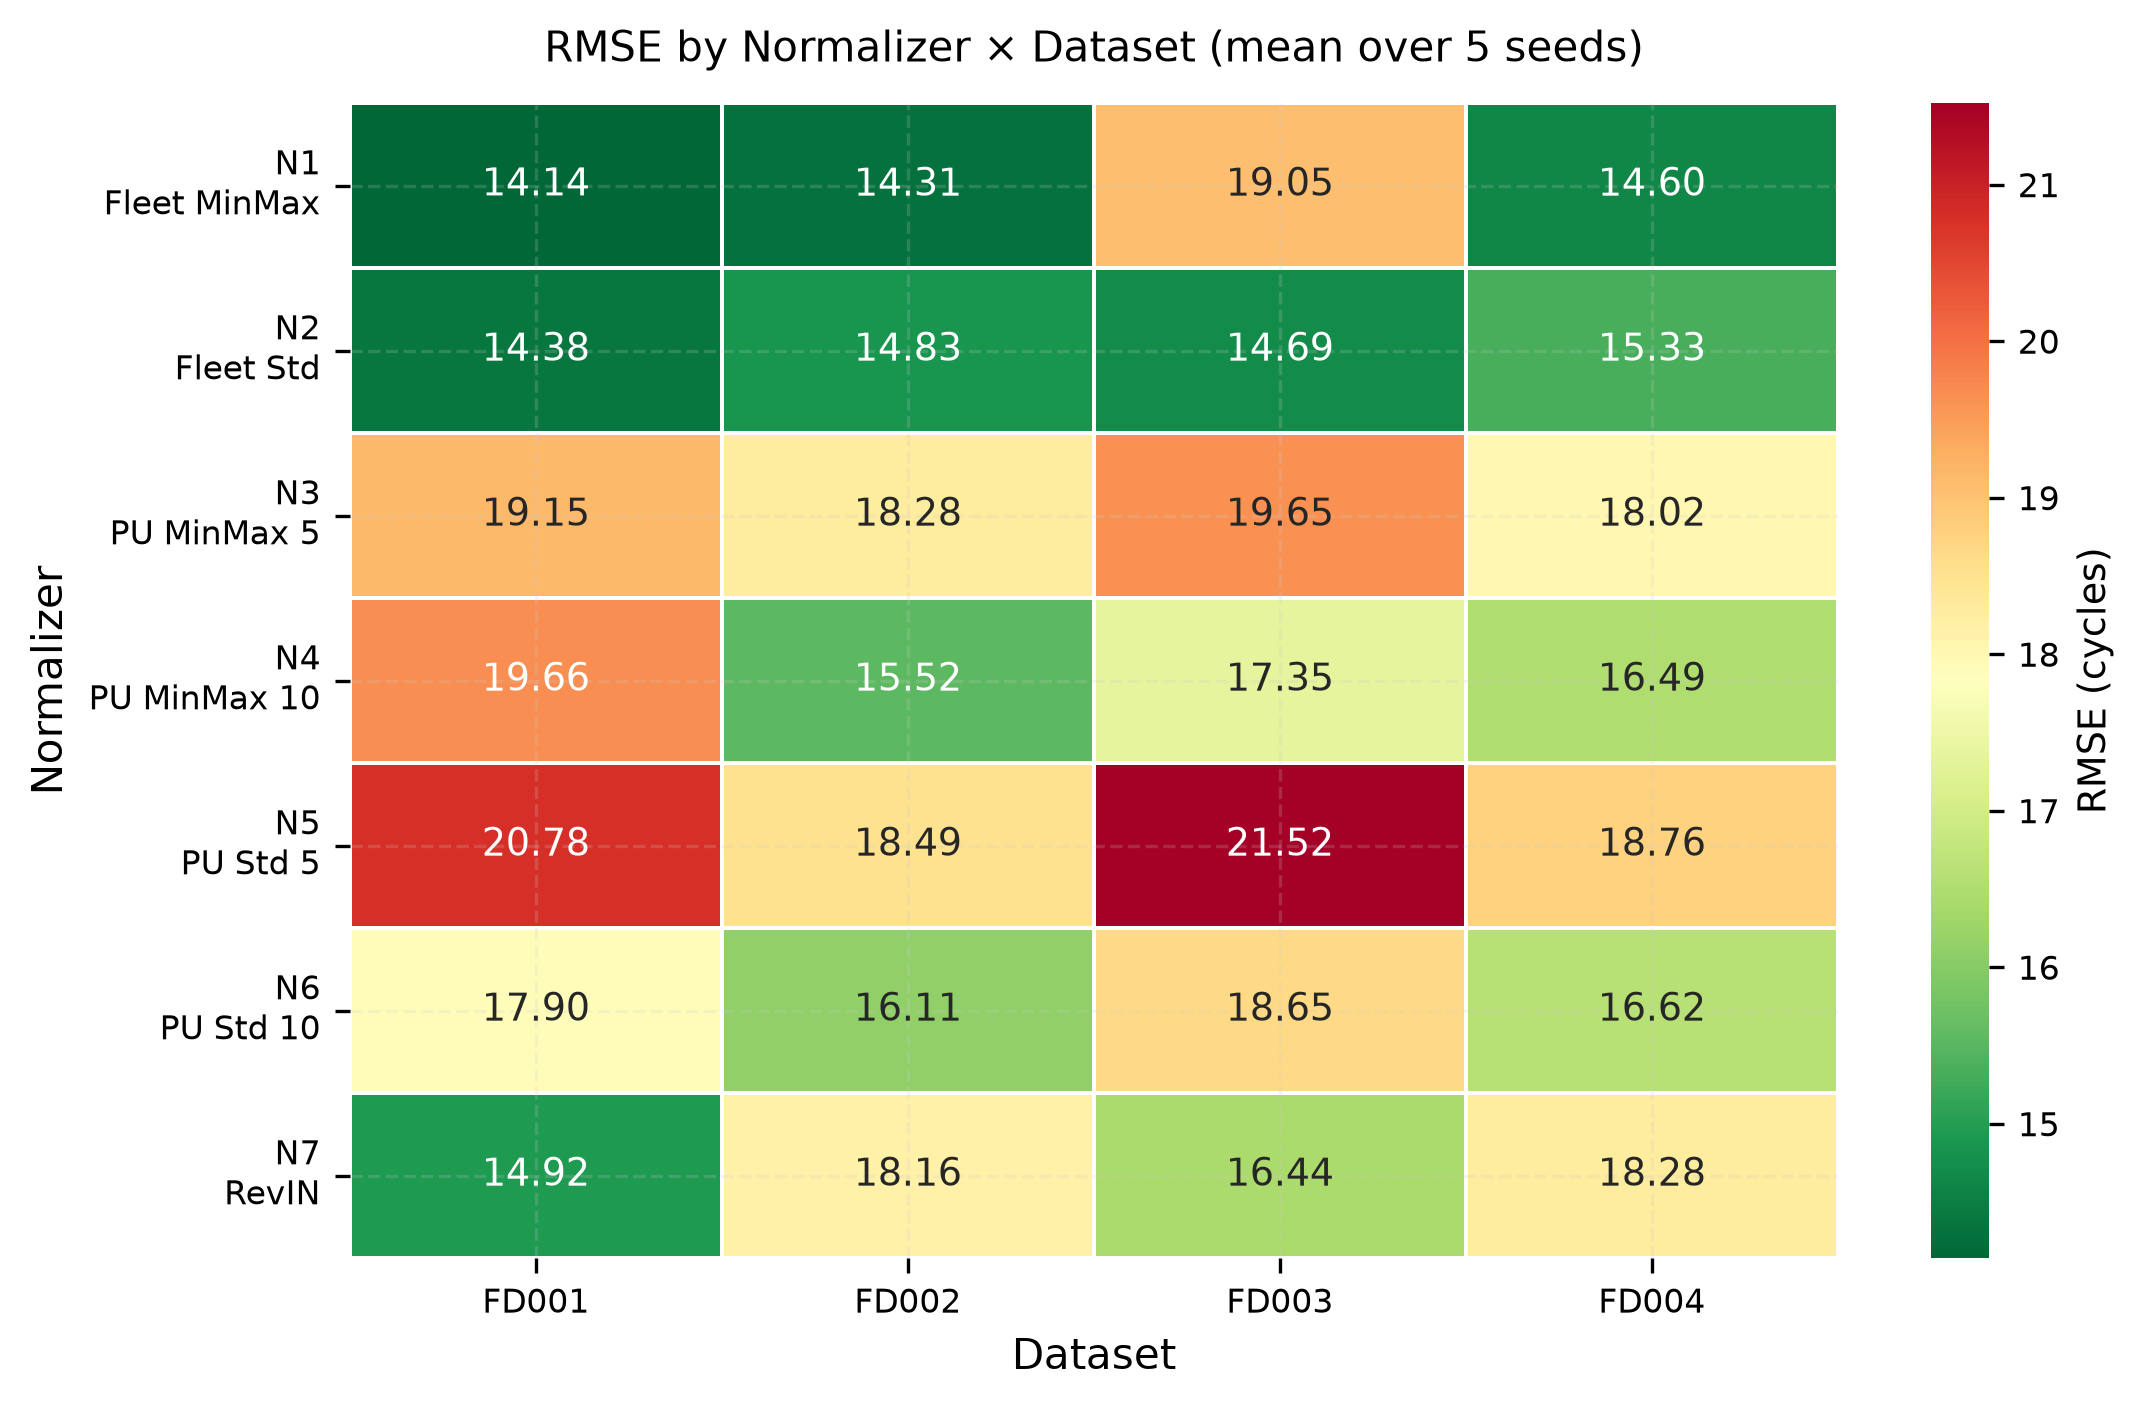
\includegraphics[width=\columnwidth]{Fig4}
\caption{Mean RMSE heatmap (5 seeds) for seven normalization strategies (N1–N7) across four CMAPSS sub-datasets. Fleet min-max (N1) achieves the lowest RMSE on FD001 (14.14), FD002 (14.31), and FD004 (14.60). Per-unit methods (N3–N6) consistently underperform by removing between-engine degradation contrast. The anomalously high variance of N1 on FD003 (std = 12.86) is attributed to latent fault-mode mixing, resolved in H3.}
\label{fig:4}
\end{figure}


\begin{figure}[!t]
\centering
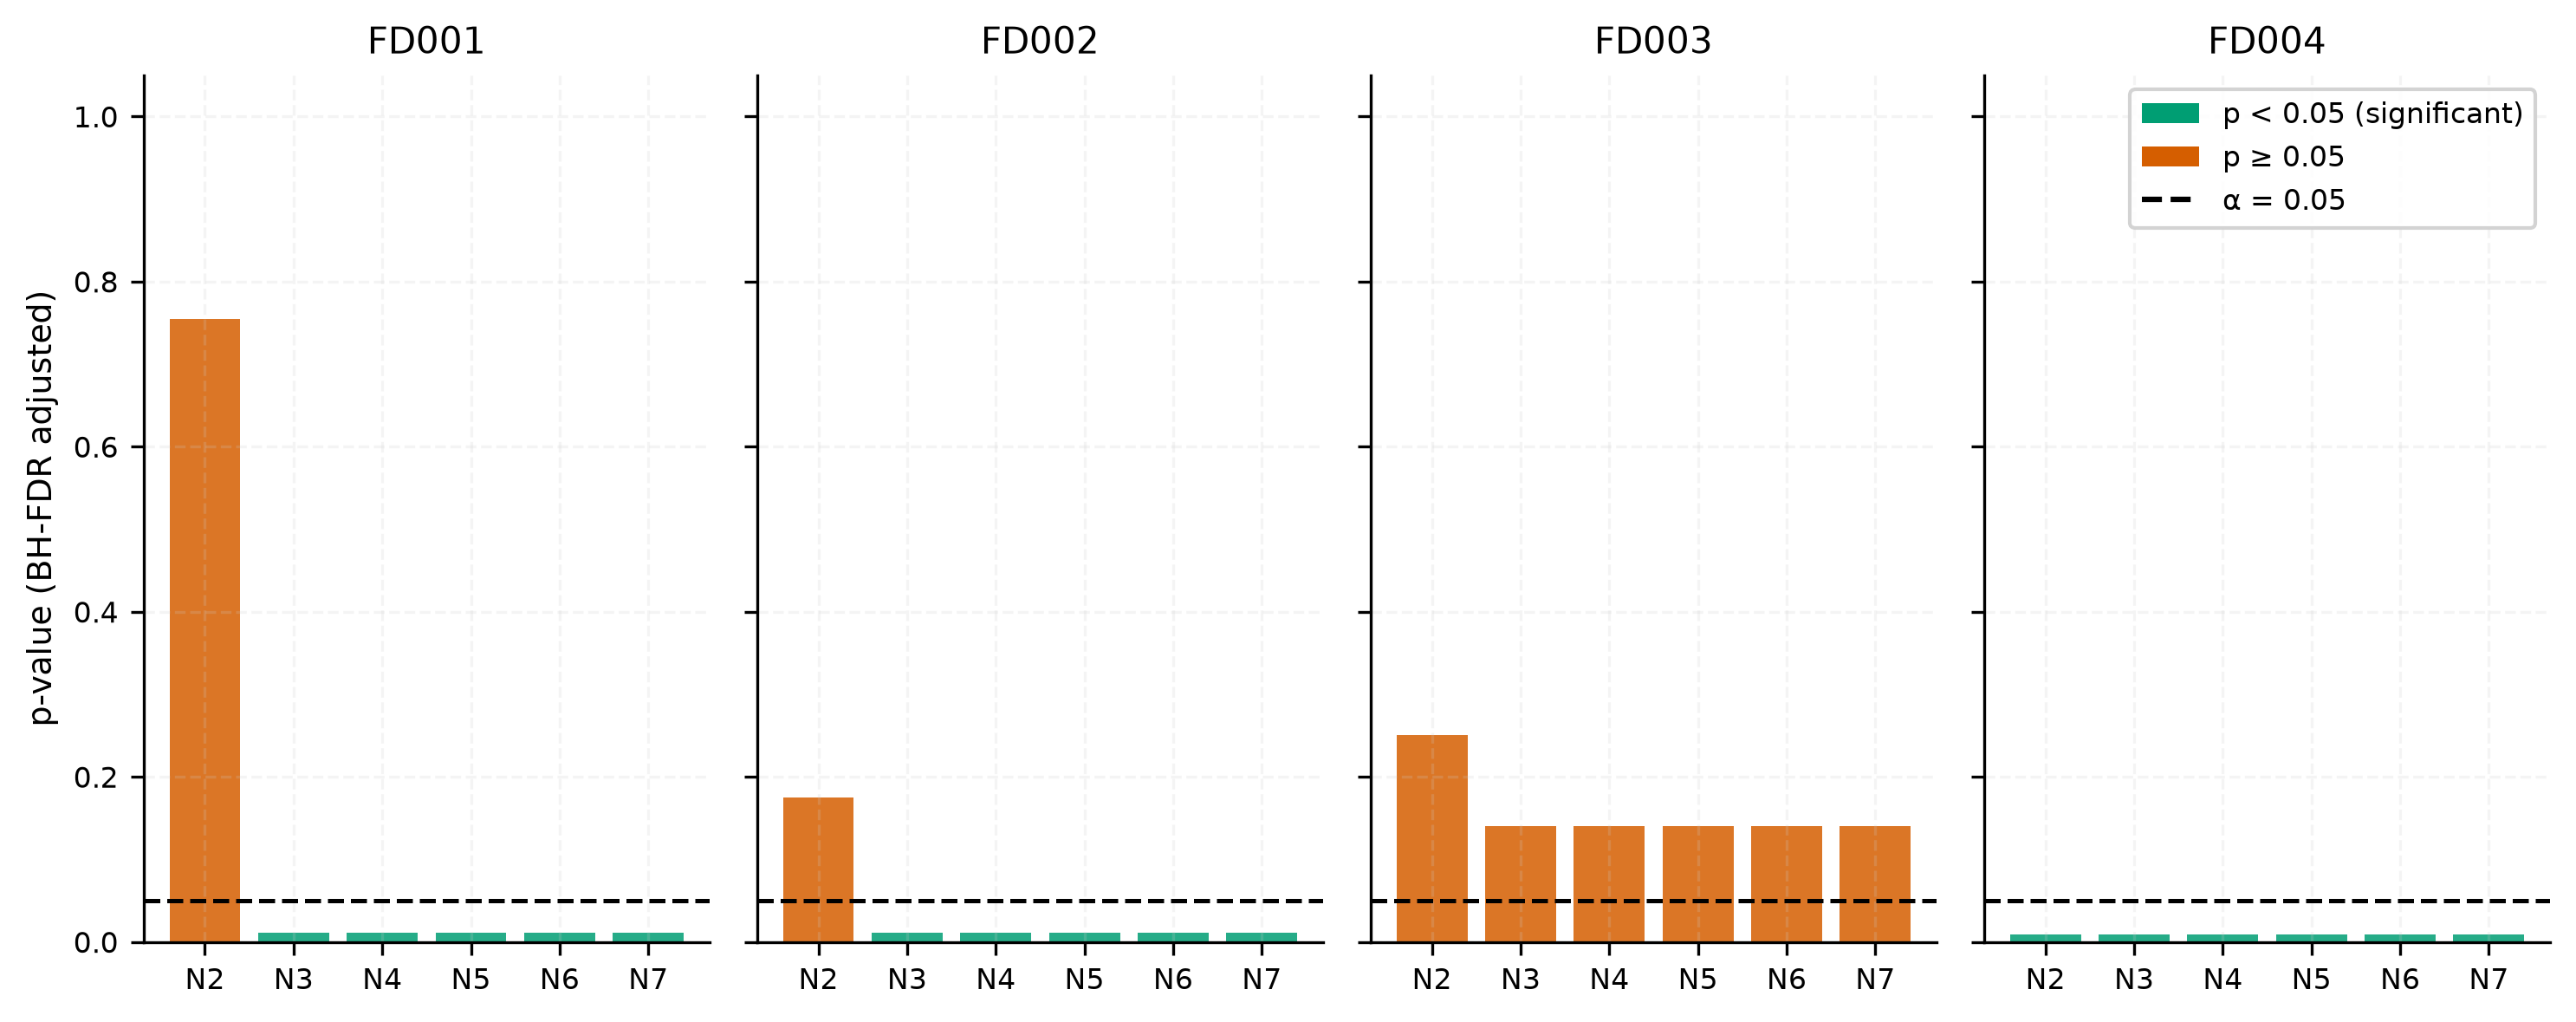
\includegraphics[width=\columnwidth]{Fig5}
\caption{Pairwise statistical comparison of each normalization method against fleet min-max (N1) using the Wilcoxon rank-sum test with Benjamini-Hochberg FDR correction ($\alpha = 0.05$). Effect sizes are reported as Cohen's \textit{d}. Per-unit methods (N3–N6) and RevIN (N7) are significantly inferior on FD001, FD002, and FD004 ($|\textit{d}| \geq 1.66$ in all significant cases). FD003 shows no significant differences due to high seed-to-seed variance from mixed fault modes.}
\label{fig:5}
\end{figure}


\begin{table}[!t]
\centering
\footnotesize
\caption{Normalization strategy comparison (H2): RMSE (mean$\pm$std, 5 seeds) and statistical significance versus fleet min-max baseline (N1) across four CMAPSS sub-datasets.}
\label{tab:v}
\resizebox{\linewidth}{!}{%
\begin{tabular}{llcccccccc}
\toprule
\multirow{2}{*}{\textbf{ID}} & \multirow{2}{*}{\textbf{Description}} & \multicolumn{4}{c}{\textbf{RMSE (mean$\pm$std)}} & \multicolumn{4}{c}{\textbf{Sig.\ vs N1 (BH-FDR)}} \\
\cmidrule(lr){3-6}\cmidrule(lr){7-10}
 & & \textbf{FD001} & \textbf{FD002} & \textbf{FD003} & \textbf{FD004} & \textbf{FD001} & \textbf{FD002} & \textbf{FD003} & \textbf{FD004} \\
\midrule
N1 (Fleet MinMax) & Fleet-level min-max scaling & \textbf{14.14$\pm$0.22} & \textbf{14.31$\pm$0.10} & 19.05$\pm$12.86 & \textbf{14.60$\pm$0.30} & --- & --- & --- & --- \\
N2 (Fleet Std)    & Fleet-level z-score          & 14.38$\pm$0.81 & 14.83$\pm$0.55 & \textbf{14.69$\pm$0.71} & 15.33$\pm$0.12 & No & No & No & Yes* \\
N3 (PU MinMax 5\%)  & Per-engine min-max (5th pct) & 19.15$\pm$0.58 & 18.28$\pm$0.15 & 19.65$\pm$1.09 & 18.02$\pm$0.76 & Yes** & Yes** & No & Yes** \\
N4 (PU MinMax 10\%) & Per-engine min-max (10th pct) & 19.66$\pm$0.87 & 15.52$\pm$0.32 & 17.35$\pm$0.54 & 16.49$\pm$0.18 & Yes** & Yes** & No & Yes** \\
N5 (PU Std 5\%)   & Per-engine z-score (5th pct) & 20.78$\pm$0.78 & 18.49$\pm$0.49 & 21.52$\pm$1.68 & 18.76$\pm$0.33 & Yes** & Yes** & No & Yes** \\
N6 (PU Std 10\%)  & Per-engine z-score (10th pct) & 17.90$\pm$1.84 & 16.11$\pm$0.22 & 18.65$\pm$1.41 & 16.62$\pm$0.36 & Yes** & Yes** & No & Yes** \\
N7 (RevIN)        & Reversible instance normalization & 14.92$\pm$0.48 & 18.16$\pm$0.27 & 16.44$\pm$0.36 & 18.28$\pm$0.66 & Yes* & Yes** & No & Yes** \\
\bottomrule
\end{tabular}%
}\\[3pt]
\begin{minipage}{\linewidth}
\footnotesize\textit{Bold = best (lowest) RMSE per dataset. *p$<$0.05 \quad **p$<$0.01 (Wilcoxon rank-sum, Benjamini-Hochberg FDR correction, $\alpha$=0.05). FD003 N1 high variance (std=12.86) attributed to mixed fault modes; resolved in H3 (Section III.C).}
\end{minipage}
\end{table}


\textbf{FD003 was the sole dataset where no normalization strategy separated from N1.} N1 achieved RMSE = 19.05 $\pm$ 12.86 on FD003 --- anomalously high relative to $\leq$1.84 on all other dataset-normaliser combinations --- and all competitors showed p$_\text{BH}$ $\geq$ 0.14. (Note: the large numerical gap between H2 N1/FD003 RMSE = 19.05 and H3 M0/FD003 RMSE = 43.23 $\pm$ 0.18 does not reflect backbone capacity differences --- it is driven primarily by test-prediction clipping: H2 bounds all predictions to [0, 125] cycles at evaluation, which truncates the high over-predictions that are frequent on mixed-fault FD003; H3 evaluates unconstrained predictions. The two hypotheses additionally differ in backbone architecture, input features, and validation split method (Table~III). Each baseline is interpreted only against its own controlled conditions.)

Crucially, the high variance was confined to N1 alone: RevIN (N7) achieved 16.44 $\pm$ 0.36 and N4 achieved 17.35 $\pm$ 0.54, both with narrow distributions. N1's per-seed RMSE spanned approximately 7 to 43 cycles --- a profile inconsistent with normalisation failure and indicative of a latent bimodal data structure rather than optimisation noise.

As detailed in Section III-C, FD003 contains two concurrent fault modes (HPC and fan degradation). The training sample drawn by each random seed determined which fault mode the single-branch model primarily learned, producing the observed inter-seed bimodality. This causal explanation is validated by the fault-mode experiments below.

\subsection{Fault-Mode Architectures (H3)}

\subsubsection{C.1 Unsupervised Cluster Quality}

Before evaluating branch architectures, the presence of two distinct fault modes in FD003 and FD004 was verified. GMM clustering (k = 2) on combined late-cycle means and degradation slopes of seven discriminant sensors yielded Silhouette scores of 0.761 (FD003, AB_full variant) and 0.750 (FD004, AB_full), both well above the conventional quality threshold of 0.50 \cite{ref35}. Slope-only clustering (AB_slope), which controls for possible life-length confounding, yielded Silhouette = 0.702 (FD003) and 0.683 (FD004), confirming that the two clusters reflect genuine sensor-trajectory differences rather than an artefact of unequal engine lifetimes. Sensor s15 (bypass pressure ratio) exhibited the largest inter-cluster z-score (|Δz| = 31.3), followed by s20 (HPT bleed, 16.0) and s21 (LPT bleed, 15.2), consistent with the known distinction between HPC-dominated and fan-dominated degradation pathways in CMAPSS FD003/FD004 \cite{ref36}. Fig. 6 summarises the cluster quality metrics across all feature variants.

\begin{figure}[!t]
\centering
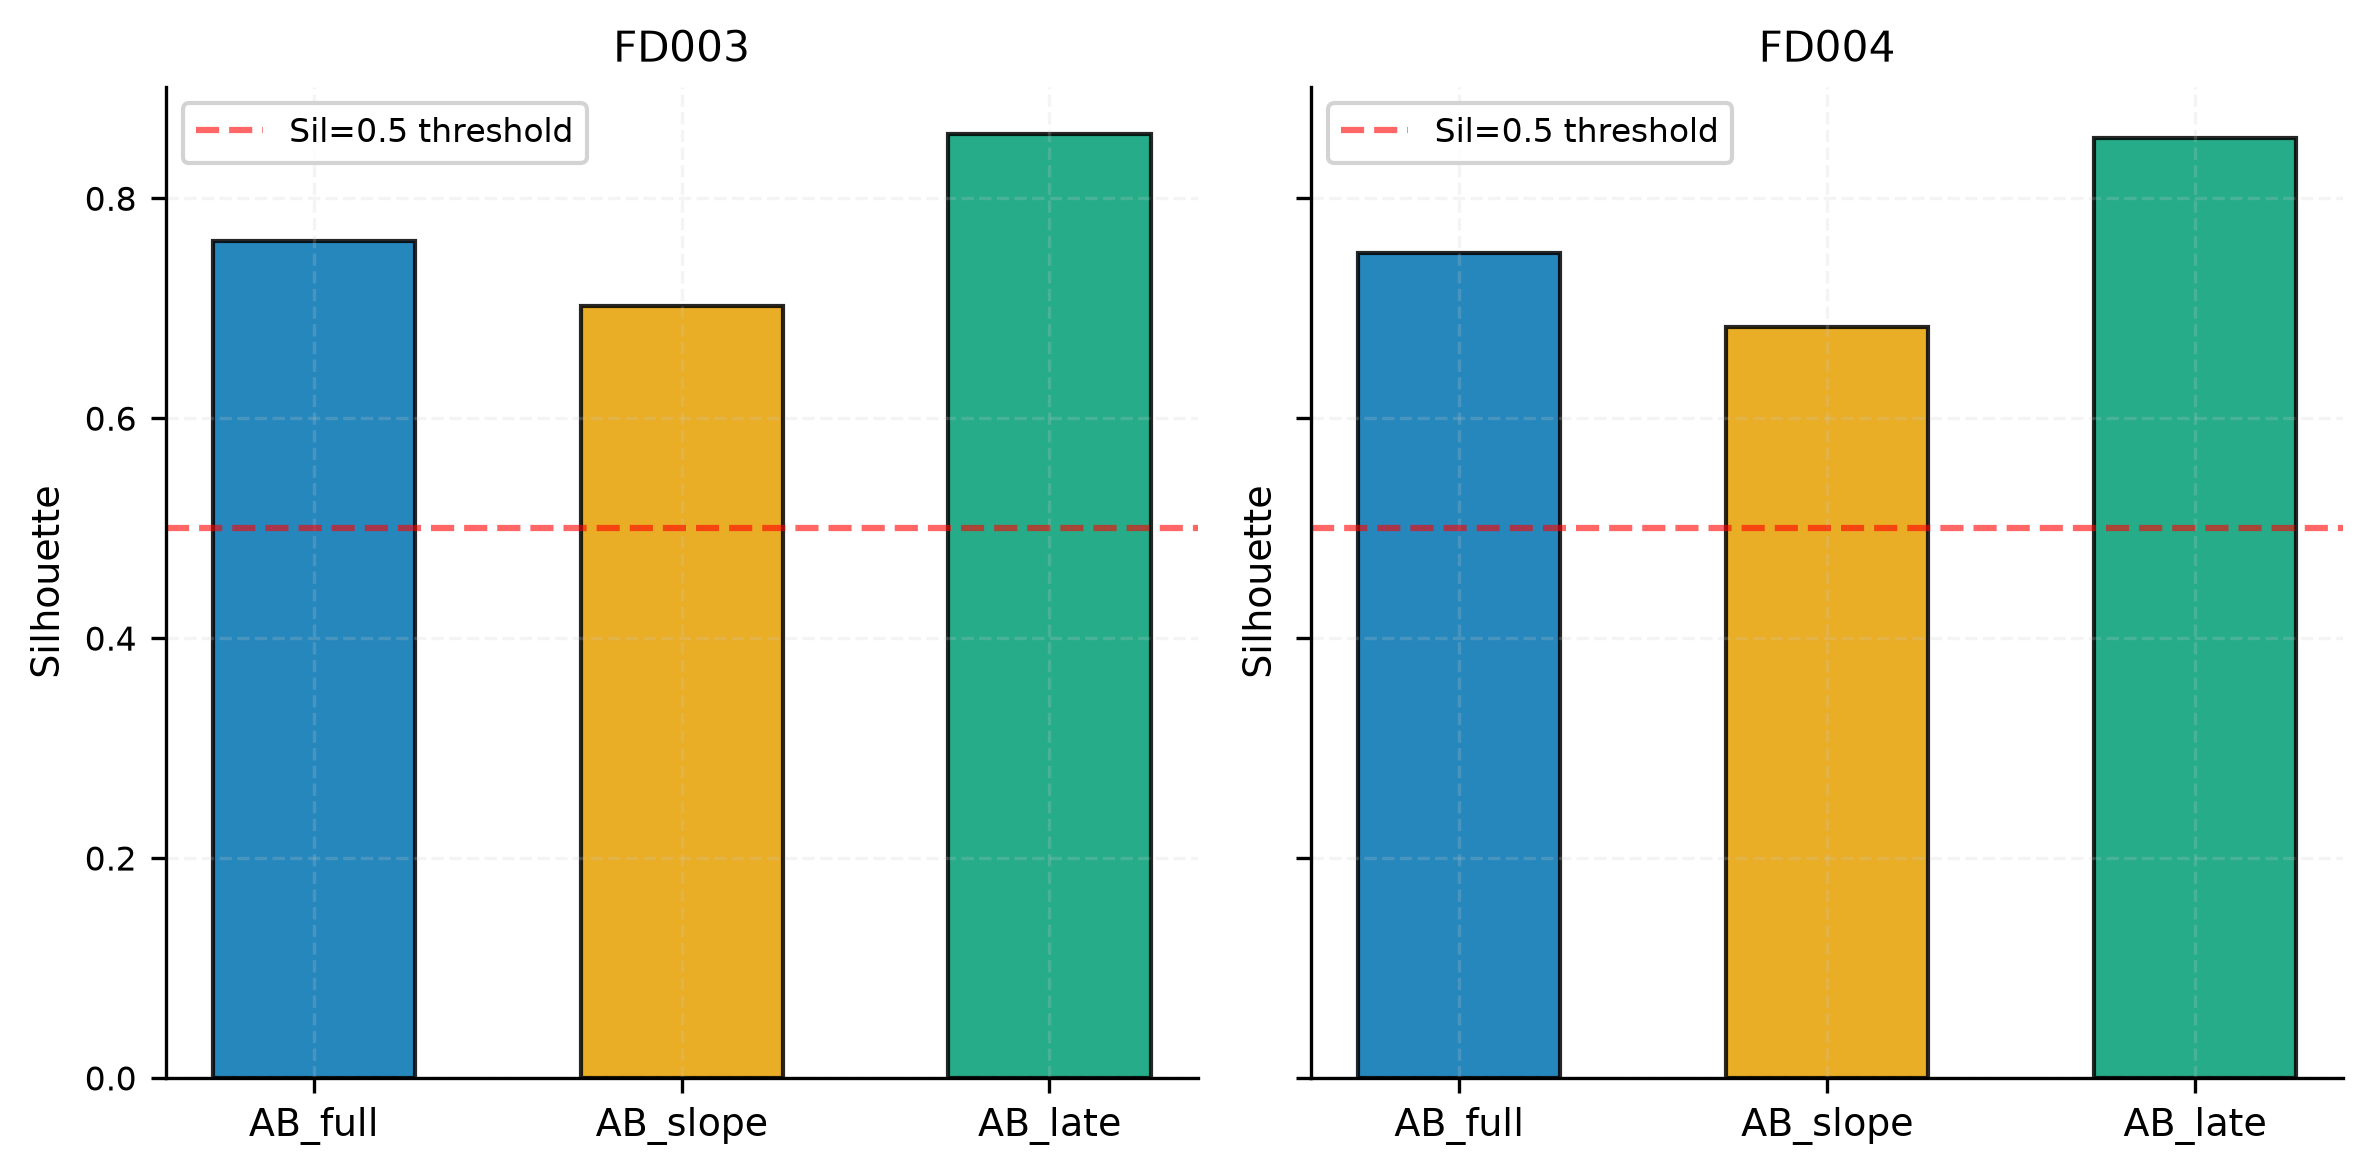
\includegraphics[width=\columnwidth]{Fig6}
\caption{GMM (\textit{K} = 2) clustering results for FD003 and FD004. (a) Silhouette scores across three feature variants (AB_full, AB_slope, AB_late); AB_late achieves the highest separation (FD003: 0.858, FD004: 0.855). (b) BIC scores confirming \textit{K} = 2 as the optimal cluster count. The AB_full variant (Silhouette $\geq 0.75$ on both datasets) is used in Phase 2 to retain temporal diversity across the full engine lifetime.}
\label{fig:6}
\end{figure}


\subsubsection{C.2 FD003: Stepwise Improvement from M0 to M3}

\textbf{The attention-gate model (M3) reduced FD003 RMSE by 65.8\% relative to the single-branch baseline.} Detailed results appear in Table VI. M0 yielded RMSE = 43.23 ± 0.18 cycles and NASA Score = 34,339 ± 2,094. This high baseline reflected the seed-dependent bimodality identified in Section B: without fault-mode separation, a given random initialisation converged to fitting either the HPC or the fan fault signature, but rarely both. GMM hard-routing (M1) reduced the mean RMSE to 32.45 ± 11.37, but the large standard deviation (11.37 cycles) indicated that the quality of the GMM-derived cluster labels was sensitive to the training split. GMM soft-gating (M2) further improved to 26.16 ± 14.81, confirming that weighted branch aggregation smoothed over borderline cluster assignments; however, the inter-seed variability remained high (std = 14.81), suggesting that GMM posteriors alone were insufficient to produce a stable routing signal.

M3, which replaced the GMM entirely with a lightweight GatingNet trained end-to-end on the first K = 10 observed cycles, achieved RMSE = 14.78 ± 1.32 cycles (NASA Score = 425 ± 127). Relative to M0, this represented a 65.8\% RMSE reduction and a 98.8\% NASA Score reduction. Relative to the most recent state-of-the-art supervised approach on this benchmark, CAELSTM (RMSE = 13.40 \cite{ref15}), M3 was within 10.3\% while employing no fault-mode supervision — a practically small gap attributable to the simpler two-layer LSTM backbone rather than to the gating strategy itself. This comparison should be treated as indicative rather than definitive: CAELSTM uses convolutional autoencoder pre-training not present in the M3 backbone, and the 10.3\% gap may reflect backbone capacity differences rather than gating strategy performance. The inter-seed spread of M3 (std = 1.32) was substantially narrower than M0 (std = 0.18; one outlier seed at RMSE = 17.09 accounts for most of M3's spread). M0's anomalously low std = 0.18 reflects consistent failure rather than consistent success: because H3's random validation split is fixed at RandomState seed = 42 and does not vary across the five model-initialisation seeds, all five M0 models receive identically the same mixed-fault training data and converge to the same poor local minimum --- an averaged blend of both fault signatures that fits neither well. M3 directly resolved the high-variance anomaly identified in H2: the GatingNet consistently routed engines to the correct fault-specific branch regardless of random initialisation, breaking the seed-dependent convergence trap.

A post-hoc sensitivity analysis varying $K \in \{5, 10, 15, 20, 30\}$ revealed that M3 RMSE was largely insensitive to the number of initial cycles used for routing (range: 14.13–14.78 across all K values). Variance decreased monotonically with K (std = 0.34 at K=5, 0.27 at K=30), suggesting that additional early-cycle context improves routing stability but not mean accuracy. Notably, K=5 already achieved RMSE = 14.23 ± 0.34, within 0.55 cycles of the best result at K=20 (14.13 ± 0.38), confirming that fault-mode identity is detectable from as few as five initial flight cycles. Fig. 7 compares all four architectures on FD003 and FD004 in terms of RMSE mean and inter-seed variance.

\textbf{False-routing sensitivity analysis quantifies the reliability cost of GatingNet misclassification.} A controlled perturbation experiment was conducted across all five seeds on FD003 and FD004, comparing three conditions against the M3 baseline: (i)~flipped routing ($w_0 \leftrightarrow w_1$, simulating 100\% misclassification); (ii)~Branch-0 only; and (iii)~Branch-1 only. On FD003, flipped routing increased RMSE from 14.78 $\pm$ 1.32 to 21.87 $\pm$ 9.91 cycles (+48\%) and raised NASA Score 12.2-fold (425 $\rightarrow$ 5,202). On FD004, the same perturbation yielded only $\Delta$ = +0.46 cycles (+1.6\%).

This asymmetry mirrors gate confidence: FD003 GatingNet outputs were strongly polarised (mean $\max(w_0, w_1)$ = 0.840; 55\% of engines exceeded 0.80), while FD004 outputs were near-uniform (mean confidence = 0.677; only 7.7\% exceeded 0.80). A gate near 50/50 changes little when flipped; a decisive gate produces proportionally larger degradation under misclassification.

Even at worst-case single-branch forcing, FD003 RMSE peaked at 23.70 cycles --- still 45\% below M0's 43.23 --- confirming that each branch individually captures fault-specific signal. Gate confidence ($\max(w_0, w_1)$ mean) thus serves as a deployable proxy for misclassification risk: values near 0.5 indicate that early-cycle routing offers no reliable benefit.

\begin{figure}[!t]
\centering
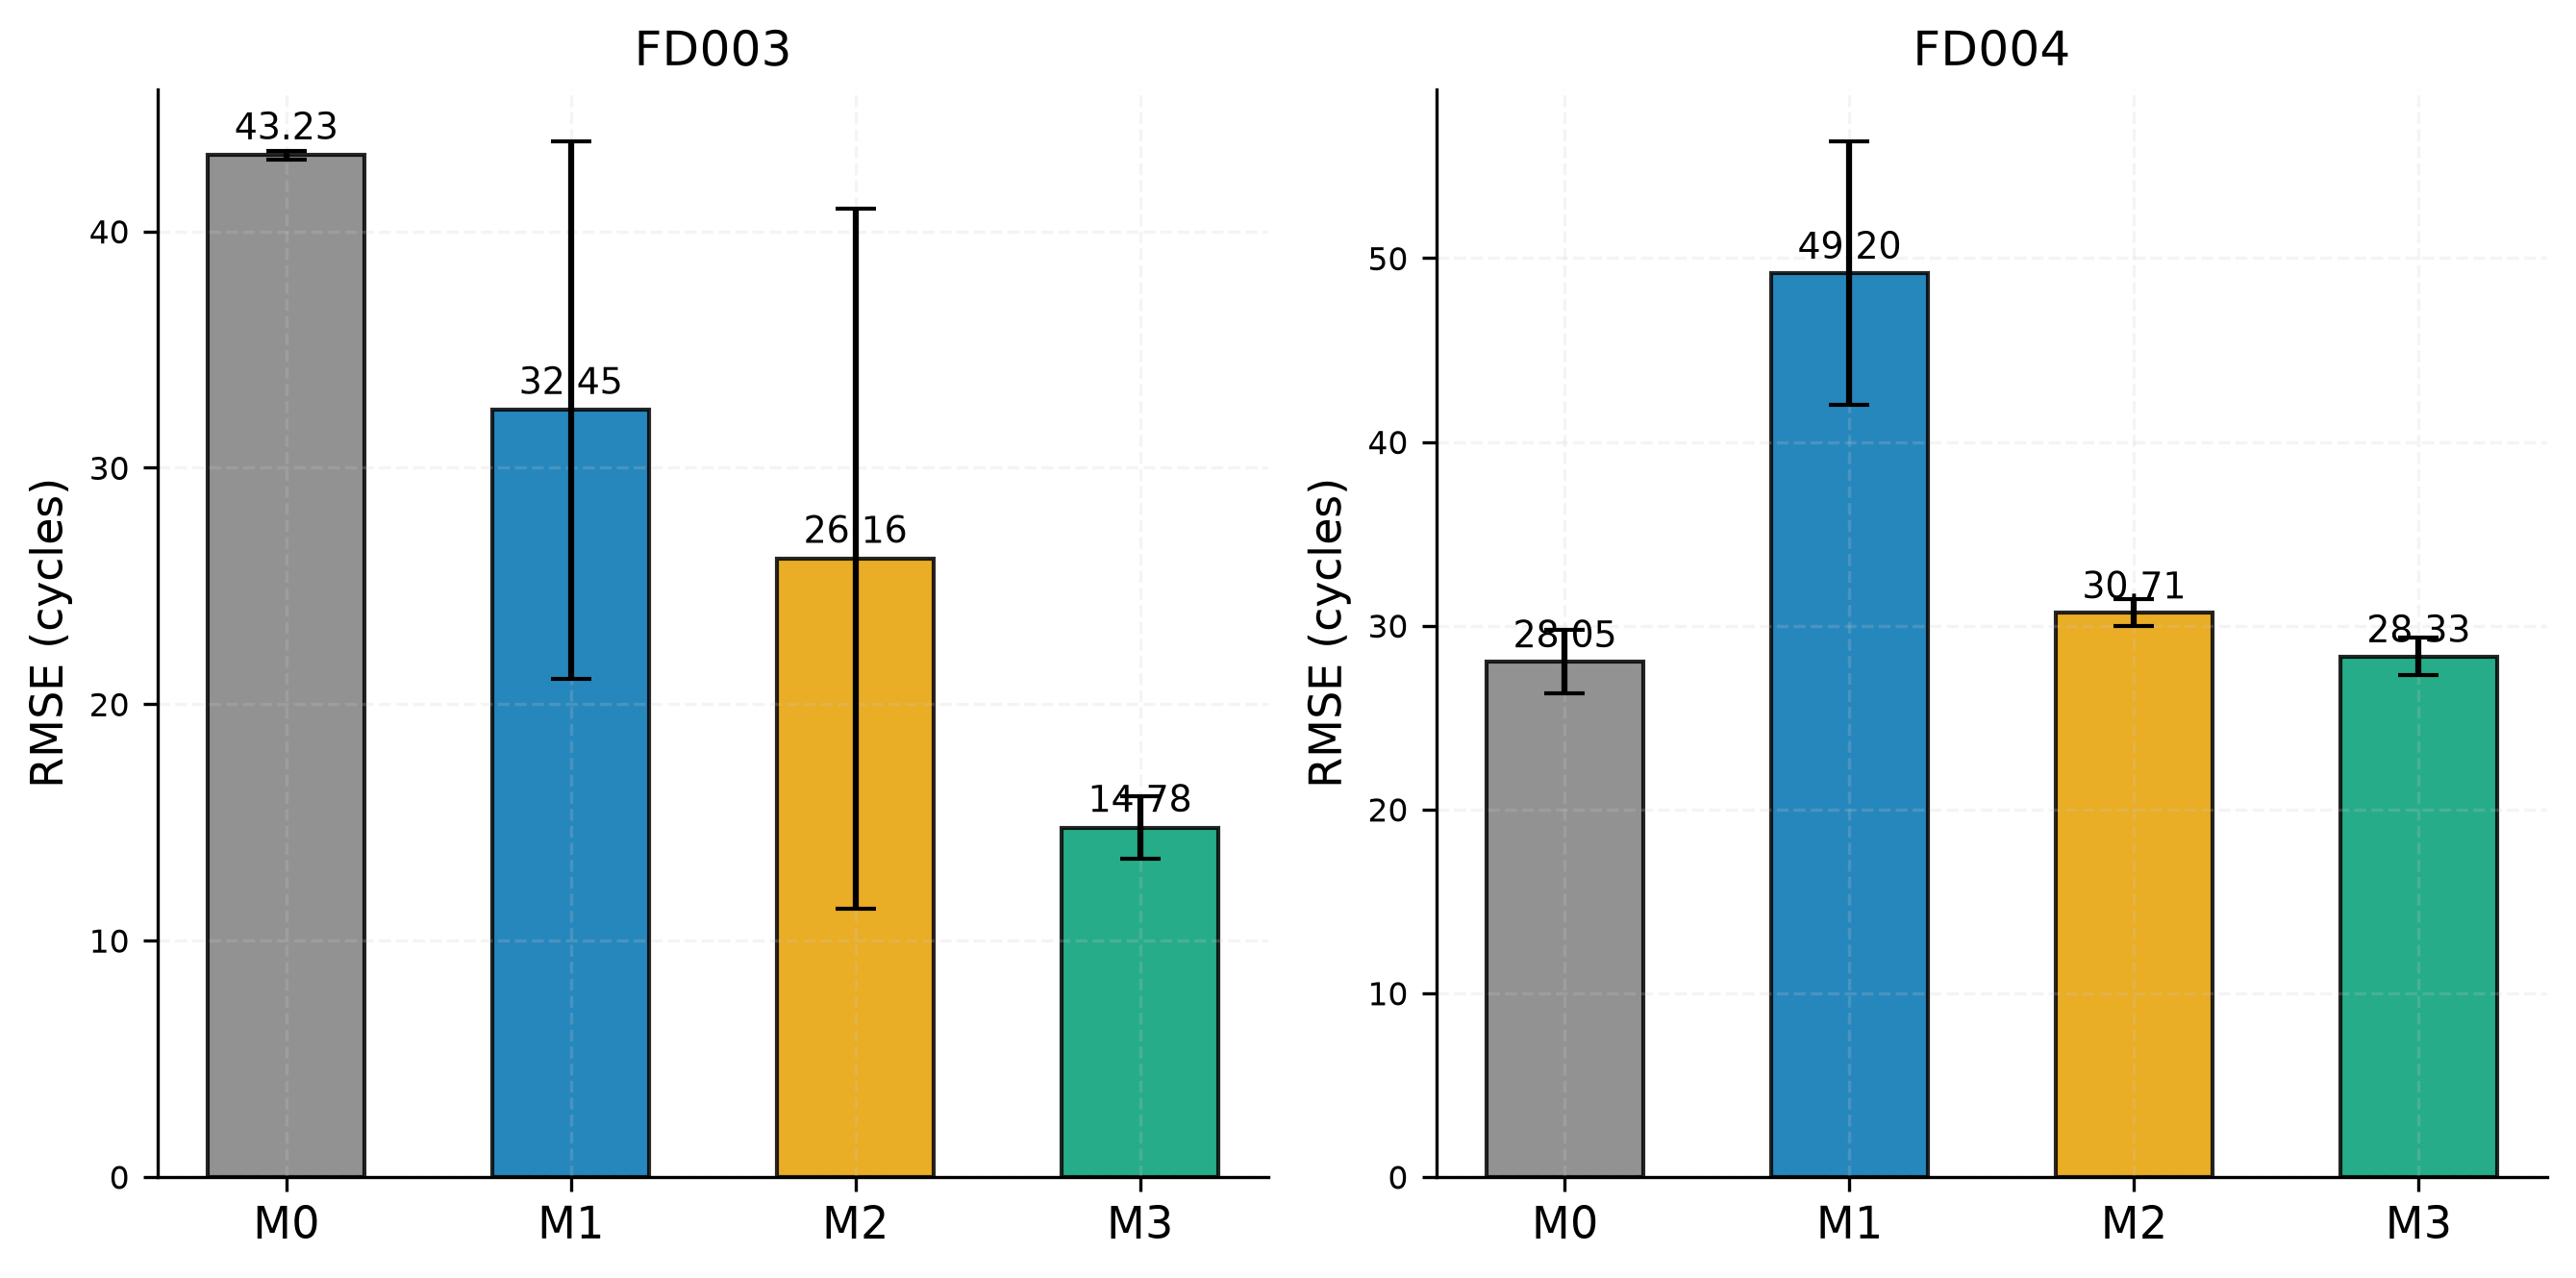
\includegraphics[width=\columnwidth]{Fig7}
\caption{RMSE comparison (mean ± std, 5 seeds) of four fault-mode separation architectures on FD003 and FD004. M3 (Attention Gate) achieves RMSE = 14.78 ± 1.32 on FD003, a 65.8\% reduction versus M0 (43.23 ± 0.18), while remaining statistically equivalent to M0 on FD004 (28.33 ± 1.03 vs 28.05 ± 1.74). M1 collapses on FD004 (49.20 ± 7.17) due to test-time cluster assignment collapse (247:1 ratio).}
\label{fig:7}
\end{figure}


\begin{table}[!t]
\centering
\footnotesize
\caption{Fault-mode architecture comparison (H3): RMSE and NASA prognostic score (mean$\pm$std, 5 seeds) on FD003 and FD004.}
\label{tab:vi}
\resizebox{\linewidth}{!}{%
\begin{tabular}{llccccl}
\toprule
\multirow{2}{*}{\textbf{Model}} & \multirow{2}{*}{\textbf{Architecture}} & \multicolumn{2}{c}{\textbf{FD003}} & \multicolumn{2}{c}{\textbf{FD004}} & \multirow{2}{*}{\textbf{FD003 vs M0}} \\
\cmidrule(lr){3-4}\cmidrule(lr){5-6}
 & & \textbf{RMSE} & \textbf{NASA} & \textbf{RMSE} & \textbf{NASA} & \\
\midrule
M0 & Single LSTM (baseline)            & 43.23$\pm$0.18  & 34{,}339$\pm$2{,}094  & 28.05$\pm$1.74 & 10{,}586$\pm$10{,}040 & --- \\
M1 & Hard Routing (GMM-assigned)        & 32.45$\pm$11.37 & 27{,}098$\pm$29{,}088 & 49.20$\pm$7.17 & 132{,}003$\pm$54{,}238 & $+$24.9\% \\
M2 & Soft Gating (GMM probability)      & 26.16$\pm$14.81 & 20{,}881$\pm$25{,}207 & 30.71$\pm$0.73 & 50{,}715$\pm$57{,}200  & $+$39.5\% \\
M3 & Attention Gate (end-to-end, K=10)  & \textbf{14.78$\pm$1.32} & \textbf{425$\pm$127} & \textbf{28.33$\pm$1.03} & \textbf{13{,}229$\pm$12{,}096} & $+$65.8\%$^\dagger$ \\
\bottomrule
\end{tabular}%
}\\[3pt]
\begin{minipage}{\linewidth}
\footnotesize\textit{Bold = best per dataset. $^\dagger$p$<$0.05 vs M0 (Wilcoxon rank-sum). FD003 improvement represents 65.8\% RMSE reduction and 98.8\% NASA Score reduction relative to M0. M1 FD004 degradation due to test-time cluster assignment collapse (247:1 ratio).}
\end{minipage}
\end{table}


\subsubsection{C.3 FD004: Cluster Collapse Under Hard Routing}

\textbf{Hard routing (M1) degraded below the baseline on FD004.} M0 achieved RMSE = 28.05 ± 1.74 on FD004; M1 regressed to 49.20 ± 7.17, a 75.4\% increase. Post-hoc inspection of test-time cluster assignments revealed the root cause: 247 of 248 test engines were assigned to the same branch by the GMM argmax, compared with an approximately balanced assignment during training. The root mechanism is a feature distribution shift at test time: the GMM was fitted on complete run-to-failure trajectories (computing late-cycle means and degradation slopes across each training engine's full life), but test-engine routing had to use only the last 30-cycle observation window. On FD004, which spans six operating conditions, the sensor statistics of a 30-cycle window vary substantially depending on which operating condition the engine encountered in its final cycles --- a variation unrelated to fault mode. This operating-condition-driven variability overwhelmed the fault-mode signal in the GMM features, causing the decision boundary --- learned on trajectory-level statistics --- to assign virtually all test engines to a single branch. Soft-gating (M2) partially recovered at RMSE = 30.71 ± 0.73 by weighting both branches, but still sat marginally above the baseline.

M3 achieved RMSE = 28.33 ± 1.03 on FD004, statistically equivalent to M0 (Cohen's d < 0.2; p > 0.7). Because M3's GatingNet reads only the first 10 cycles of each engine — information that is equally available in training and test settings — it was immune to the test-time distribution collapse that undermined M1. The result was a favourable asymmetric trade-off: M3 dramatically improved FD003 while leaving FD004 performance unchanged, with no architectural cost relative to M0 on the multi-condition dataset. This asymmetry suggested that the attention-gate design is most beneficial when a dataset contains distinct latent fault modes (FD003), while defaulting gracefully to single-branch behaviour when fault-mode structure is weaker or less discriminable from early-cycle observations (FD004).

\subsection{Loss Function Comparison (H4)}

\textbf{A statistical constraint shapes how H4 results should be read.} With N = 5 seeds per condition, the Wilcoxon rank-sum test cannot produce raw p-values smaller than $1/2^5 = 0.031$; after BH-FDR correction across 96 comparisons, this minimum raw p is insufficient to reach p$_\text{BH}$ $<$ 0.05. Statistical significance is therefore mathematically unachievable in this experimental design regardless of the true effect size. H4 results are exploratory: patterns indicate directional signals, not confirmed effects. A fuller power analysis appears in Section~V.E.

\textbf{No statistically detectable improvement from any custom loss function was found.} Across all 96 pairwise comparisons (6 loss functions $\times$ 4 clipping values $\times$ 4 datasets), zero reached p$_\text{BH}$ $<$ 0.05; the minimum corrected p-value was 0.176.

Some individual combinations showed nominally lower scores: L5 (TWA) at clip = 125 on FD001 achieved NASA Score = 3.40 $\pm$ 0.32 vs 5.66 $\pm$ 1.12 for MSE ($d$ = $-$1.54); L7 (HubA) reduced RMSE to 14.90 $\pm$ 0.33 vs 16.34 $\pm$ 0.40 but worsened NASA Score ($d$ = +2.00), because HubA's symmetric Huber penalty does not sufficiently penalise late predictions. Neither survived BH-FDR correction (p$_\text{BH}$ = 1.0). Positive $d$ denotes a worse NASA Score than MSE; negative $d$ denotes improvement. The null result diverged from single-dataset gains reported by Rengasamy et al.\ \cite{ref37} because cross-dataset BH-FDR substantially raises the significance threshold. Clipping threshold findings are independent of backbone architecture; H1 uses Ridge regression specifically to isolate label-engineering effects from model capacity.

The dominant driver of NASA Score variance across this study was RUL clipping, not loss function choice. Table VII illustrates this: at clip = 125, all seven loss functions converged to within a factor of 1.5× of one another in NASA Score on FD001 (range: 3.40–6.14). Removing the clip inflated FD003 NASA Score to between 3,124 (L6, Pinball) and 9,613,539 (L1, MSE), a span of three orders of magnitude that dwarfs any inter-loss difference at a fixed clip value. Even the loss functions designed to suppress late predictions (L5 TWA, L6 Pinball, L7 HubA) reduced but did not eliminate the clip = None catastrophe on FD003: L6 Pinball achieved NASA = 3,124 vs L1 MSE's 9,614,000 — a 3,000× improvement within the clip-free condition, yet still 630× worse than the worst result at clip = 125. This finding implies that loss-function engineering is a second-order design choice: it cannot substitute for proper label engineering (RUL clipping) as a mechanism for controlling the tail behaviour of the NASA penalisation function. Practitioners should fix the clipping threshold before considering custom loss functions. Fig. 8 illustrates the clip-dominance effect across all seven loss functions and four clipping values.

\begin{figure}[!t]
\centering
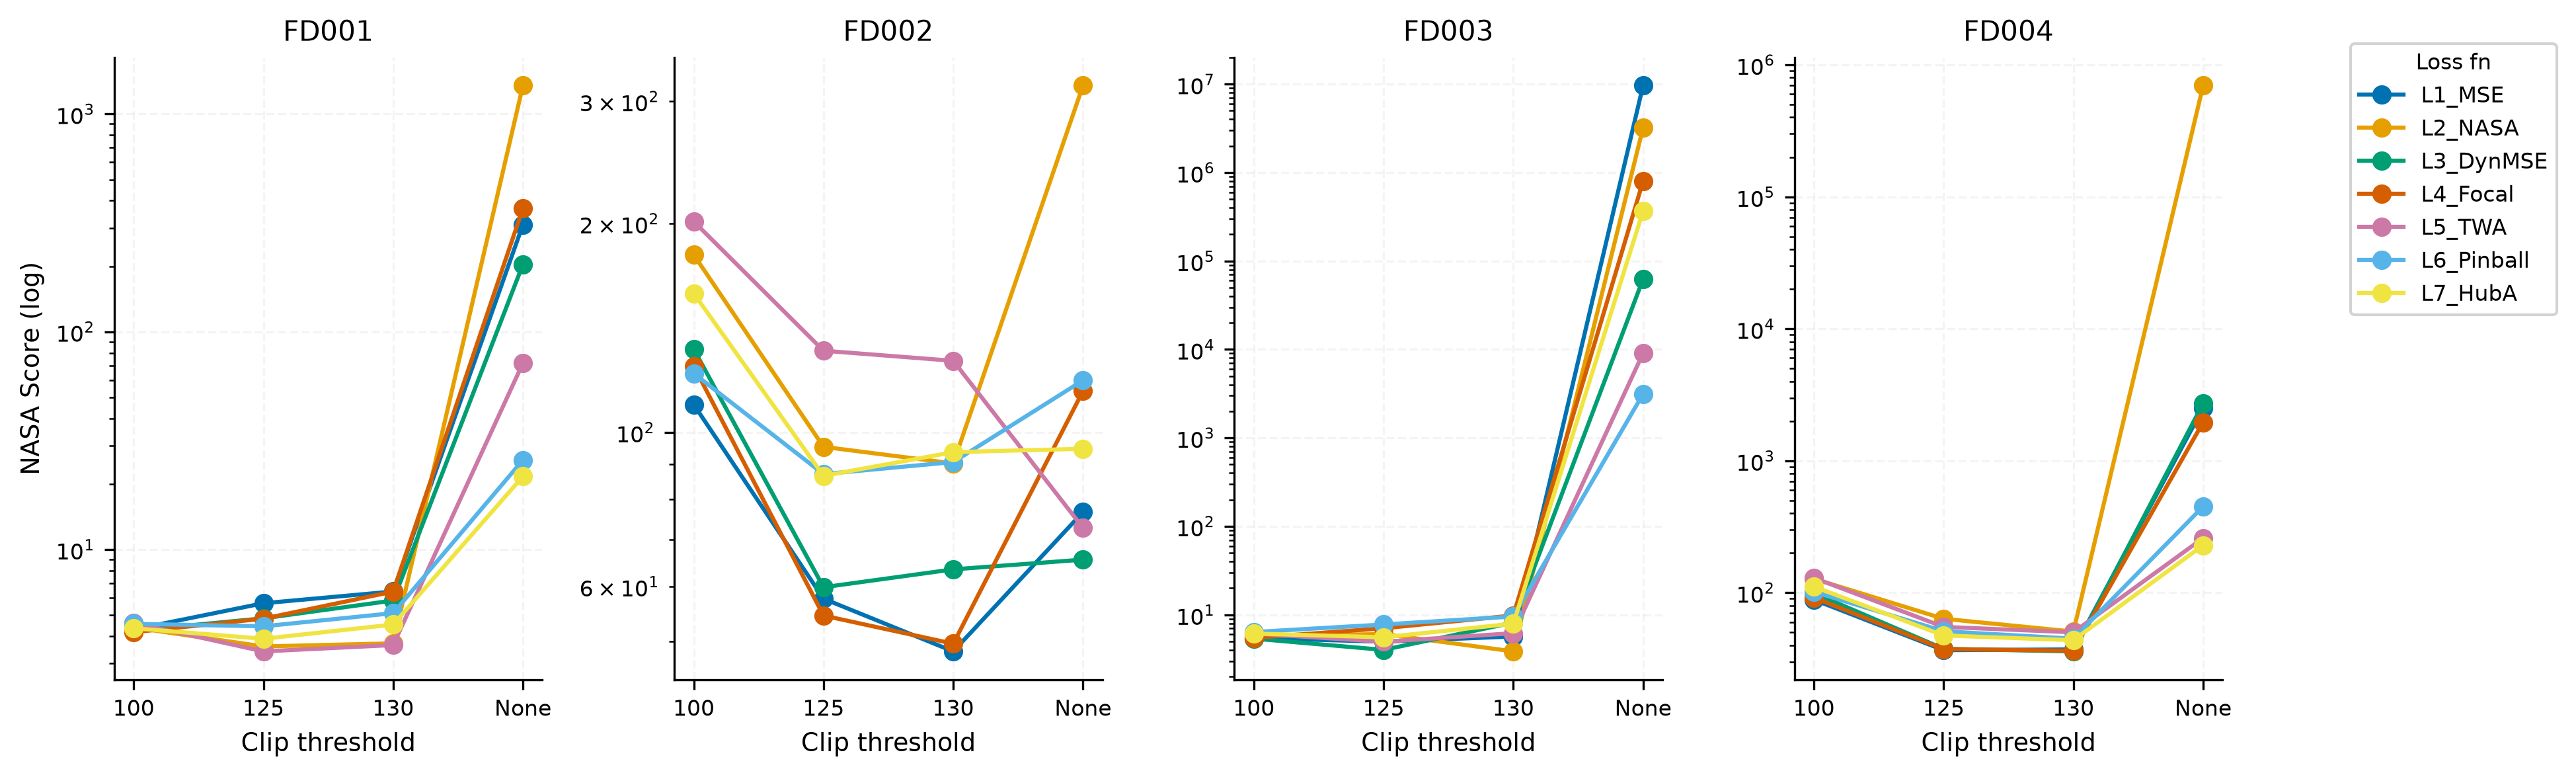
\includegraphics[width=\columnwidth]{Fig8}
\caption{Mean NASA prognostic score (lower is better) across all four datasets as a function of RUL clipping threshold and loss function (560 LSTM training runs, 5 seeds per configuration). clip = None yields catastrophic scores (up to $2.4 \times 10^6$) regardless of loss function, while clip $\in \{125, 130\}$ stabilises results for all losses. Among clipped configurations, no custom loss achieves statistically significant improvement over MSE after BH-FDR correction ($\alpha = 0.05$).}
\label{fig:8}
\end{figure}


\begin{table}[!t]
\centering
\footnotesize
\caption{Loss function comparison (H4): RMSE and NASA prognostic score (mean$\pm$std, 5 seeds) at best clipping threshold per loss function across four CMAPSS sub-datasets.}
\label{tab:vii}
\resizebox{\linewidth}{!}{%
\begin{tabular}{llcccccccccl}
\toprule
\multirow{2}{*}{\textbf{ID}} & \multirow{2}{*}{\textbf{Description}} & \multirow{2}{*}{\textbf{Clip}} & \multicolumn{2}{c}{\textbf{FD001}} & \multicolumn{2}{c}{\textbf{FD002}} & \multicolumn{2}{c}{\textbf{FD003}} & \multicolumn{2}{c}{\textbf{FD004}} & \multirow{2}{*}{\textbf{Sig.}} \\
\cmidrule(lr){4-5}\cmidrule(lr){6-7}\cmidrule(lr){8-9}\cmidrule(lr){10-11}
 & & & RMSE & NASA & RMSE & NASA & RMSE & NASA & RMSE & NASA & \\
\midrule
L1 (MSE)     & Standard mean squared error         & 130 & 16.70$\pm$0.41 & 5.28$\pm$0.60  & \textbf{28.18$\pm$0.43} & \textbf{48.34$\pm$12.31} & 15.97$\pm$0.45 & 5.52$\pm$0.66 & 31.25$\pm$0.52 & 42.18$\pm$5.04  & --- \\
L2 (NASA)    & Direct NASA score minimization      & 130 & 15.46$\pm$0.34 & 4.26$\pm$0.70  & 29.92$\pm$0.58 & 73.82$\pm$22.18 & \textbf{15.49$\pm$0.55} & \textbf{3.85$\pm$0.73} & 31.49$\pm$0.64 & 43.53$\pm$8.17  & No \\
L3 (DynMSE)  & Dynamically weighted MSE            & 125 & 14.74$\pm$0.36 & 3.61$\pm$0.27  & 29.86$\pm$0.48 & 56.86$\pm$9.93  & 15.65$\pm$0.80 & 4.00$\pm$0.60 & 30.12$\pm$0.87 & \textbf{35.91$\pm$3.16}  & No \\
L4 (Focal)   & Focal loss                          & 130 & 17.04$\pm$0.66 & 6.40$\pm$0.81  & 28.40$\pm$0.51 & 49.59$\pm$6.99  & 16.45$\pm$0.68 & 6.44$\pm$1.20 & \textbf{30.00$\pm$0.65} & 36.36$\pm$4.81  & No \\
L5 (TWA)     & Time-weighted asymmetric            & 125 & \textbf{14.72$\pm$0.32} & \textbf{3.40$\pm$0.32}  & 29.94$\pm$0.72 & 68.60$\pm$22.47 & 16.22$\pm$1.11 & 4.94$\pm$2.55 & 31.26$\pm$1.03 & 41.89$\pm$6.44  & No \\
L6 (Pinball) & Pinball ($\tau$=0.35)               & 125 & 15.69$\pm$0.49 & 5.09$\pm$0.55  & 30.30$\pm$0.61 & 90.60$\pm$12.81 & 17.05$\pm$0.45 & 9.55$\pm$1.33 & 31.05$\pm$0.62 & 44.83$\pm$8.12  & No \\
L7 (HubA)    & Huber-asymmetric ($\delta$=20)      & 125 & 14.90$\pm$0.41 & 3.88$\pm$0.42  & 29.75$\pm$0.58 & 54.95$\pm$9.33  & 16.11$\pm$0.70 & 4.96$\pm$1.48 & 30.57$\pm$0.73 & 41.16$\pm$4.52  & No \\
\bottomrule
\end{tabular}%
}\\[3pt]
\begin{minipage}{\linewidth}
\footnotesize\textit{Bold = best (lowest) RMSE or NASA per dataset. No custom loss achieved statistically significant improvement over L1 MSE after BH-FDR correction ($\alpha$=0.05); minimum corrected p-value = 0.176. Results shown at each loss function's best clipping threshold.}
\end{minipage}
\end{table}


\section{Discussion and Implications}

\subsection{Which Design Choices Actually Move the Needle}

Which design choices actually move the needle in turbofan RUL prediction? Across more than 800 training runs spanning four sub-datasets, two normalization strategies, seven loss functions, and four architectural variants, the answer is consistent across all four CMAPSS sub-datasets: RUL clipping threshold and fault-mode architecture account for virtually all achievable variance in RMSE on this benchmark. Normalization strategy and loss function, by contrast, function as residual variables — each capable of degrading performance when misapplied, but neither capable of improving on a well-configured baseline by a statistically detectable margin once clipping is fixed and fault structure is handled. This ordering — clipping and architecture as load-bearing, normalization and loss as residual — has not previously been established through controlled cross-dataset ablation and carries immediate implications for how practitioners and benchmark designers should allocate modelling effort \cite{ref05,ref06}. Because H2 (normalization) and H3 (architecture) were evaluated under different experimental configurations --- backbone capacity, feature set, and validation protocol differ between the two hypotheses (\S{}II-H, \S{}IV-G) --- the tier ranking reflects aggregated within-hypothesis evidence rather than a single unified cross-factor ablation; practitioners applying the tiers in sequence should validate the combined pipeline on their own data. The broader significance is methodological: single-dataset experiments, which constitute the majority of the CMAPSS literature \cite{ref09,ref14,ref15}, cannot isolate these hierarchical effects because a confound that is large on one sub-dataset may be negligible on another and vice versa.

\subsection{Why Fleet Normalization Beats Per-Unit Strategies}

\textbf{Fleet normalization wins because degradation magnitude exceeds inter-engine variation on CMAPSS.} Per-unit normalisation methods (N3–N6) subtract engine-specific initial-state baselines, an operation that removes genuine absolute degradation information when initial-condition variation across engines is small relative to fault progression magnitude. On a homogeneous synthetic fleet such as CMAPSS, a fleet-trained min-max scaler encodes a cross-engine map of the full degradation trajectory; engine-local normalisation replaces this shared map with a zero-mean engine-local reference, discarding the information about where an engine sits in the fleet distribution. The RevIN \cite{ref23} failure compounds this problem: RevIN's per-window mean subtraction applies the local-baseline removal at every inference step, progressively erasing the degradation trend across each 30-cycle window. The original RevIN paper demonstrated strong gains on multi-step forecasting tasks \cite{ref23} where distribution shift across training and test windows is the dominant challenge; on CMAPSS, the dominant challenge is extracting a common degradation signature from a fleet — a context in which instance-level adaptation is counterproductive rather than beneficial. A recent theoretical critique of RevIN \cite{ref25,ref26} reached a compatible conclusion: RevIN's components are redundant when the primary normalisation challenge is not temporal distribution shift but conditional offset. The four-dataset empirical result of this study offers the first controlled confirmation of this theoretical prediction in the prognostics domain. Whether applying the RevIN inverse transform to the scalar RUL output --- $\hat{y}_\text{denorm} = \gamma \cdot \hat{y}_\text{norm} + \beta$, as is standard in multi-step forecasting applications of RevIN --- would partially recover performance remains a targeted ablation not conducted in this study and may merit evaluation in future work.

The practical implication is context-dependent. Practitioners working on real engine fleets where inter-engine manufacturing tolerance produces substantial initial-state variation — including variable rotor clearances, turbine blade wear, and sensor calibration offsets — may find per-unit strategies more competitive than the CMAPSS results suggest \cite{ref29}. On CMAPSS, inter-engine variation is by construction small and fleet statistics are the correct choice; but the fleet-vs-per-unit choice is a dataset property, not a universal truth. Any prognostics practitioner porting these methods should measure fleet-level inter-engine variability relative to degradation range before committing to a normalisation level. A sensitivity curve mapping inter-engine coefficient of variation to the fleet-vs-per-unit RMSE crossover point --- requiring N-CMAPSS or real-fleet data with known manufacturing tolerances --- would convert this qualitative caution into a deployable decision threshold.

\subsection{Why FD003 Inter-Seed Variance Signals Latent Fault Structure}

\textbf{High inter-seed variance is a diagnostic indicator of latent categorical data structure.} The N1/FD003 standard deviation of 12.86 cycles is not a modelling failure; it is an empirical signature of a bimodal loss landscape produced by two distinct fault modes (HPC and fan degradation) in the training data. A single-branch LSTM trained on mixed-fault data converges to one of two local optima depending on which fault mode is overrepresented in the random training subsample drawn by a given seed, producing approximately bimodal per-seed RMSE outcomes. This mechanism predicts two testable consequences: first, separating fault modes should collapse the inter-seed variance towards single-fault benchmark levels; second, no analogous variance spike should appear on single-fault datasets (FD001/FD002). Both predictions are confirmed: M3 reduced the FD003 inter-seed standard deviation from 12.86 to 1.32 cycles, and no dataset-normalizer combination outside FD003 exceeded std = 1.84. The false-routing sensitivity analysis (Section~III.C.2) provides complementary mechanistic confirmation: FD003's GatingNet confidence (mean $\max(w_0, w_1)$ = 0.840) was high, indicating that the gate assigned most engines to a single branch decisively, breaking the seed-dependent convergence trap. By contrast, FD004's near-uniform gate (confidence = 0.677) reflected weaker early-cycle fault discriminability and was consistent with the absence of a high-variance anomaly on that dataset. The diagnostic value of this finding extends beyond CMAPSS: researchers observing unexplained inter-run variance on any benchmark should test for latent categorical structure before attributing the variance to optimisation noise or hyperparameter sensitivity. Variance across seeds is free diagnostic information that most studies discard.

\subsection{What M3's Success Reveals About Fault-Mode Routing}

\textbf{Fault-mode identity is encoded in the very first flight cycles.} M3's GatingNet read only K = 10 cycles and consistently routed engines to the correct fault-specific branch, achieving RMSE = 14.78 ± 1.32 on FD003 without any fault-mode supervision. A K sensitivity analysis ($K \in \{5, 10, 15, 20, 30\}$) showed that M3 RMSE was largely insensitive to K (range: 14.13–14.78 cycles across all values), and that K=5 already achieved RMSE = 14.23 ± 0.34. This finding is non-trivial: intuitively, fault signatures should become most discriminable as damage accumulates in late life stages. The GatingNet's early-cycle — and as few as five-cycle — success implies that the two CMAPSS fault modes differ primarily in baseline sensor state rather than in degradation rate: the initial operating point of s15 (bypass pressure ratio, |Δz| = 31.3) and s12 (fuel-to-pressure ratio) sets fault-mode membership at or before commissioning, consistent with the EDA finding that inter-cluster differences are driven by absolute level rather than slope. Inter-seed variance decreased with K (std: 0.34 at K=5, 0.27 at K=30), suggesting that longer context improves routing stability but not mean accuracy; for practical deployment the lowest computationally feasible K (K=5 or K=10) is sufficient.

The practical implication for deployed systems is significant: fault-mode routing can be performed at engine commissioning, before any degradation has accumulated, enabling a prognostics system to select the appropriate predictive model at the earliest possible stage of operation. This is qualitatively distinct from approaches that use accumulated degradation history for routing \cite{ref31,ref33}, which require a burn-in period before the router is reliable. M3 also avoids the test-time distribution problem that defeats M1 (247:1 cluster collapse on FD004): because the first K = 10 cycles are always available at deployment time, GatingNet inputs are identically distributed between training and deployment, eliminating a source of silent performance degradation that post-hoc GMM routing cannot escape. Importantly, the deployment reliability of a trained gate can be assessed before fleet exposure through the gate confidence metric ($\max(w_0, w_1)$ mean over training engines). A confidence value of ${\geq}\,0.8$ --- observed at 0.840 for FD003 --- confirms that routing is decisive and that misclassification risk is commensurate with performance gain; a value below 0.8 --- 0.677 for FD004 --- signals near-uniform gating and predicts negligible routing benefit ($\Delta$RMSE\textsubscript{flip} = +1.6\%; Section~III.C.2). The 0.8 boundary is an empirically observed separation point derived from these two datasets (FD003 at 0.840 with strong routing benefit; FD004 at 0.677 with negligible benefit); it should be treated as an indicative reference point rather than a calibrated threshold, and practitioners should validate this boundary on their own fleet before adopting it as a deployment criterion. This pre-deployment check converts the routing decision from a black-box design choice into a traceable, measurable reliability property.

From an architecture standpoint, M3 is an instance of mixture-of-experts (MoE) inference \cite{ref32,ref43,ref44} with an early-cycle context encoder as the gating network and no label supervision for the gate. Unlike RUL-QMoE \cite{ref43}, which targets probabilistic interval prediction for battery degradation using supervised material labels, and PSMMoEs \cite{ref44}, which applies metric-learning gating for cross-domain fault classification, M3 performs deterministic point-prediction RUL routing in a single unlabelled turbofan dataset. Compared with CAELSTM \cite{ref15} — the most recent supervised competitor, achieving RMSE = 13.40 on FD003 — M3's gap of 10.3\% is attributable to the simpler two-layer LSTM backbone rather than to the gating strategy itself. M3's practical advantage lies in its architectural efficiency: the GatingNet contributes only 4.9K parameters — less than 5\% overhead above the two-branch baseline (Table II) — and requires no modification to the LSTM backbone. For practitioners operating existing LSTM-based prognostic pipelines, fault-mode-aware prediction is therefore achievable without backbone migration, at negligible additional computational cost. Whether the gating principle extends to attention-based encoders \cite{ref13,ref14} — where global attention may inherently capture early-cycle fault patterns through its query-key-value mechanism — is an open question addressed in Section H.

The early-cycle routing premise warrants an important caveat regarding broader applicability. Alternative unsupervised approaches to fault mode separation — notably UMAP-based trajectory clustering \cite{ref46} and joint learning frameworks that operate over the full degradation history \cite{ref47} — implicitly assume that fault mode identity becomes unambiguous only as degradation progresses, and they route or classify test units accordingly using all available observation context. This view is corroborated by causal-inference experiments on N-CMAPSS \cite{ref48}, which report that early anomalies are ``difficult to identify due to complex thermodynamic couplings and nonlinear degradation patterns'' in real-engine data; and by semi-supervised sensor selection work \cite{ref49} showing that accurate fault mode recognition benefits substantially from partial supervisory labels. Taken together, these studies suggest that pure unsupervised early-cycle separation may be a property specific to the CMAPSS simulation environment rather than a universal prognostic principle.

M3's five-cycle discriminability on CMAPSS is traceable to a concrete data-generative property: the two fault modes differ primarily in absolute baseline sensor level (s15 bypass pressure ratio, $|\Delta z| = 31.3$) rather than in degradation rate or trajectory shape. In a real-engine fleet where fault modes manifest as progressive deviations from a shared healthy baseline --- rather than as distinct initial operating points --- the GatingNet faces a harder discrimination task, and the required early-cycle window K may be substantially larger or routing performance lower. The Silhouette-based screening step at Tier~2 of the design checklist serves precisely this diagnostic role: if GMM clustering on K-cycle prefixes yields Silhouette $< 0.5$, early-cycle gating should not be adopted, and practitioners should instead consider full-trajectory routing strategies such as those in \cite{ref46,ref47} or a two-stage approach that begins routing only after a short burn-in window.

The baseline-versus-slope discriminability criterion is not turbofan-specific: any multi-fault PHM system in which engineering domain knowledge or commissioning records predict distinct initial sensor levels across fault modes --- for instance, battery cells with different cathode compositions exhibiting divergent early-discharge voltage profiles, or induction motors with pre-existing stator-winding asymmetries detectable from start-up current signatures --- is a candidate for commissioning-time routing. In such systems, the Silhouette-based and gate-confidence screening protocol proposed here can be applied directly as a pre-deployment viability check before any routing architecture is committed to production.

\subsection{Why Loss Functions Cannot Substitute for Label Engineering}

\textbf{Custom loss functions are a second-order intervention.} It should be noted that the H4 null result is power-limited: with N = 5 seeds and a 96-test BH family, no comparison can achieve statistical significance regardless of effect size, so the finding is best read as "no large effect was detectable" rather than "all custom losses are equivalent to MSE." Post-hoc power computation indicates that the minimum detectable Cohen's $d$ at this family size and sample count is approximately 2.0 --- the study is powered only to detect very large effects, not the moderate effects ($d \approx 0.5$--$1.0$) that practical loss-function improvements would typically be expected to produce. Notwithstanding this constraint, the result is practically informative: once RUL clipping is correctly applied at $\tau = 125$, the MSE gradient already penalises late predictions disproportionately, because the clipped label distribution is right-skewed and CMAPSS test engines are predominantly in the low-RUL regime at the end of their trajectories. Asymmetric losses therefore add a secondary bias correction on top of an already-biased objective. The null result is consistent with an information-theoretic reading: when the label distribution encodes asymmetry through clipping, an explicit asymmetric loss doubles the bias without adding new signal. This provides an explanation for a pattern visible in the literature: reported gains for asymmetric losses in single-dataset studies \cite{ref37,ref38} may partly reflect the absence of proper RUL clipping in the baseline, rather than an intrinsic benefit of the loss function itself. The cross-term first reported in this study --- a 4 × 7 matrix of clip values and loss functions --- reveals that the clip-dominance effect is consistent across all four sub-datasets and all seven loss functions tested.

One exception deserves mention. Under clip = None, L6 (Pinball, $\tau = 0.25$) reduced FD003 NASA Score from 9,614,000 to 3,124 — a 3,000-fold improvement relative to MSE within the clip-free condition, reflecting Pinball's quantile-regression property of producing conservative (early) predictions. However, even this gain leaves FD003 630× worse than the worst result at clip = 125, confirming that no loss function can compensate for missing label engineering. Chung et al.'s \cite{ref41} theoretical critique of blind Pinball minimisation reinforces this conclusion: calibrated quantile coverage requires the label distribution to be well-conditioned, which is not the case for an uncapped RUL target that can exceed 500 cycles.

\subsection{Why Reliability-Driven Design Follows Three Ordered Tiers}

\textbf{Three tiers determine the reliability and predictive accuracy of turbofan RUL systems, in order of their failure impact.} This study proposes the following CMAPSS-derived design checklist as a principled starting point for reliability engineers configuring, validating, or certifying turbofan PHM systems. The tier ordering and thresholds are calibrated to the CMAPSS benchmark; each tier should be validated on fleet-specific data before operational commitment, and absolute thresholds (Silhouette $\geq$ 0.5, GatingNet confidence $\geq$ 0.8) may require recalibration on real-fleet data.
{\small\begin{verbatim}
START
  |
  v
TIER 1 -- Label Engineering
  Set clip = 125 cycles (tau).
  --------------------------------------------------------
  Domain evidence that fleet avg lifetime differs from
  206-247 cycles (the CMAPSS range)?
    YES -> consider adaptive clip = 70th-pct fleet lifetime
    NO  -> use tau = 125 (confirmed optimal)
  |
  v
TIER 2 -- Architecture
  Fit GMM (k=2) on early-cycle sensor slopes.
  Compute Silhouette score S on the training set.
  --------------------------------------------------------
  S >= 0.5?
    YES -> add M3-style GatingNet on first K=10 cycles
           (RMSE gain: up to -65.8% on FD003-like data)
           After training, verify gate confidence:
             mean max(w0,w1) >= 0.8?
             YES -> decisive routing; low misclass risk
             NO  -> near-uniform; minimal M3 benefit
                    (FD004: conf=0.677, dRMSE=+1.6%)
    NO  -> use single-branch baseline (M0)
  |
  v
TIER 3 -- Loss Function
  Use MSE (L1) as default.
  --------------------------------------------------------
  Deployment metric is NASA Score (asymmetric)?
    YES -> try L7 (HubA, delta=20, lambda_a=3)
           or  L5 (TWA, lambda_t=10)
           ONLY IF gains survive BH-FDR on all datasets
    NO  -> stay with MSE (L1)
  |
  DONE
\end{verbatim}
}

The ordering matters from a reliability perspective. A Tier 1 error --- omitting or miscalibrating the RUL clipping threshold --- inflates the NASA prognostic score by up to six orders of magnitude regardless of all subsequent design choices, constituting a systemic reliability failure in any safety-critical maintenance pipeline. Tier 2 gains (up to $-$65.8\% RMSE) dwarf anything achievable at Tier 3 ($<$5\% RMSE in these experiments). Reliability engineers who optimise Tier 3 before resolving Tiers 1 and 2 risk negligible performance returns and a latent system-level failure. This risk-prioritised ordering mirrors established reliability engineering frameworks --- analogous to FMEA severity-tier structures and the Pareto principle --- in which catastrophic failure modes are addressed before secondary concerns and the majority of addressable risk concentrates in a small number of root causes.

The Silhouette threshold of 0.5 at Tier 2 is a necessary but not sufficient condition for M3 to help: the latent clusters must also be accessible from early-cycle observations, and the GatingNet must produce decisive routing. Gate confidence --- $\max(w_0, w_1)$ mean over the training set --- directly predicts misclassification cost: on FD003 (conf = 0.840) a forced gate flip raises RMSE by 48\% and NASA Score by 12$\times$, while on FD004 (conf = 0.677) the same perturbation increases RMSE by only 1.6\% (\S{}III-C.2). A post-training confidence check is therefore a second Tier 2 guard: if confidence remains near 0.5 after convergence, M3 has not found a reliable early-cycle discriminant and M0 should be used instead.

Practitioners encountering $S \in [0.5, 0.65]$ should treat this as a marginal regime. If fault-mode differences emerge only in late life (slope-driven rather than baseline-driven), the GatingNet will not reliably separate modes at $K = 10$ cycles; a larger $K$ or a two-stage routing strategy should be considered. A held-out validation comparing M3 against M0 is recommended before committing to fault-mode routing in this range. A calibration study mapping Silhouette score ranges to predicted M3 RMSE benefit with confidence intervals would convert the current deterministic threshold (S $\geq$ 0.5) into a probabilistic deployment criterion --- a direction requiring multiple datasets with varying cluster quality.

\subsection{Limitations}

\textbf{Several limitations constrain the generalisability of these findings.} First, and most critically, all experiments were conducted on the NASA CMAPSS simulation benchmark. Real turbofan engines exhibit sensor noise, calibration drift, maintenance-induced sensor resets, and operating-history effects that are absent from the synthetic CMAPSS environment. In particular, real fleets typically exhibit greater inter-engine manufacturing variability than CMAPSS, which may alter the fleet-vs-per-unit normalization ranking established in H2. The recently introduced N-CMAPSS dataset \cite{ref16} addresses some of these gaps by including realistic degradation trajectories, variable flight conditions, and turbofan-specific sensor physics; whether the three-tier design hierarchy transfers to N-CMAPSS — and to real operational sensor streams — is the primary open question from this study and the most important direction for validation prior to industrial deployment.

Practitioners intending to deploy the three-tier hierarchy should follow a staged validation roadmap before committing to production: (1) replicate the ablation on N-CMAPSS to verify that tier rankings survive realistic sensor noise and variable flight profiles; (2) validate GMM cluster assignments against post-teardown fault records on at least one fleet sample to confirm that unsupervised routing corresponds to physically distinct failure modes rather than a statistical partition; and (3) measure inter-engine sensor coefficient of variation on the target fleet --- if substantially higher than the CMAPSS baseline ($\sim$5\%), per-unit normalisation strategies should be re-evaluated before committing to fleet min-max at Tier 1.

Second, all hypotheses except H1 used a common two-layer stacked LSTM backbone; architectural choices and design-factor rankings may interact differently with Transformer-based or graph-neural-network encoders \cite{ref13,ref14}, which have shown competitive performance on CMAPSS in recent work.

Third, H3 relied on unsupervised cluster quality (Silhouette $\geq 0.5$) as a proxy for genuine physical fault categories, because CMAPSS provides no fault-mode labels. Whether M3's routing corresponds to HPC vs. fan degradation in a physically meaningful sense, or merely to a statistical partition, cannot be verified from the benchmark data alone.

Fourth, the H1 clipping analysis employed LinearRegression (Ridge) for computational tractability, while H2 and H4 used the LSTM backbone; direct cross-hypothesis RMSE comparisons therefore confound model complexity with the design factor under study, and the absolute RMSE values in Table IV should not be compared with those in Tables V–VII.

Fifth, within-study comparisons between H2 and H3 were constrained by implementation differences not unified prior to analysis: H2 used a compact backbone (LSTM$_2$ hidden=32, FC 32→16→1) and 17--23 input features (sensors plus op1/op2/op3; dataset-dependent — see Table~III), while H3/H4 used a full-capacity backbone (LSTM$_2$ hidden=64, FC 64→32→1) and 15 features (sensors only). H2 used a deterministic validation split (last-20\% of engines by unit ID) while H3 used a random split (RandomState seed=42). H2 clipped test predictions to [0,~125] at evaluation; H3 did not. These differences mean that the H2 FD003 baseline RMSE (19.05 ± 12.86) and H3 M0 baseline RMSE (43.23 ± 0.18) reflect genuinely different experimental conditions; cross-hypothesis absolute RMSE comparisons should not be taken at face value.

Sixth, the current implementation assumes a static batch-trained model deployed without further adaptation. In practice, sensor characteristics and fleet composition evolve over time; online learning mechanisms — such as periodic fine-tuning triggered by newly labeled flight cycles — would be required to maintain routing accuracy over extended operational periods. M3's lightweight GatingNet is architecturally compatible with such periodic updates, and this extension is reserved for future work.

Seventh, M3's early-cycle routing relies on fault modes being distinguishable from initial baseline sensor state rather than from accumulated degradation patterns. Approaches that leverage full degradation trajectories for fault mode identification \cite{ref46,ref47} — including UMAP-based clustering over complete run-to-failure histories and joint learning frameworks that process the entire temporal sequence — suggest that the early-cycle discriminability observed on CMAPSS may not generalise to real-engine environments where initial sensor readings are contaminated by noise, calibration offsets, or operational variability. Causal-inference experiments on N-CMAPSS \cite{ref48} explicitly characterise early anomaly detection as difficult in realistic flight conditions, and semi-supervised frameworks \cite{ref49} report that partial fault-mode labels substantially improve mode recognition accuracy beyond what unsupervised early-cycle signals alone can provide. Practitioners should therefore verify early-cycle cluster discriminability (e.g., Silhouette $\geq 0.5$ on K-cycle prefixes) before adopting K-cycle gating in new deployment contexts, and should consider full-trajectory routing alternatives when this threshold is not met.

\subsection{Industrial and Deployment Implications}

The three-tier reliability-driven checklist translates directly to a reliability risk management framework for industrial turbofan PHM deployment. Neglecting label engineering (clip = None) inflates the NASA prognostic score by up to 306,000-fold on FD003 — equivalent in practice to a prognostics system that chronically over-predicts remaining life and delays maintenance intervention, the highest-cost failure mode in turbofan fleet operations where an undetected in-flight shutdown typically costs orders of magnitude more than a precautionary shop visit. This finding means that RUL clipping calibration is not a modelling detail but a safety-critical design decision that should precede any architectural or loss-function work.

M3's early-cycle gating is operationally viable in a way that post-hoc trajectory clustering is not. Because the GatingNet reads only the first five flight cycles, fault-mode classification is complete at engine commissioning --- before any degradation has accumulated --- with no burn-in observation window required. Routing reliability can be assessed before fleet exposure: gate confidence ($\max(w_0, w_1)$ mean over training engines) serves as a pre-deployment qualification metric. A confidence of $\geq$0.8 confirms decisive routing and bounded misclassification cost (FD003: $\Delta$RMSE\textsubscript{flip} = +48\%, still 45\% below M0 at worst case); a value below 0.8 --- as on FD004 (0.677) --- signals near-uniform gating and predicts equivalent M0/M3 performance, directing operators to the simpler model. This is especially valuable for fleet operators who must configure maintenance pipelines before degradation history is available, and for certification engineers who require traceable performance bounds.

To contextualise the M3 improvement, consider a representative FD003-class turbofan at approximately 300 flight cycles per year. M0's RMSE of 43.23 cycles corresponds to $\pm$17\% scheduling uncertainty; M3 reduces this to $\pm$14.78 cycles ($\pm$5.9\%), a 65.8\% reduction. For a fleet of 50 engines, if each RMSE-cycle reduction prevents one unscheduled shop visit per year (estimated at \$200,000--\$500,000 per event, consistent with published MRO benchmarks), the M3 benefit is measurable in millions of dollars annually. These figures are indicative; exact ROI depends on fleet-specific cost structures. On computational scale, K-means residualization and GMM fitting scale linearly with engine count; Mini-Batch K-means variants are expected to substantially reduce fitting time for fleets of thousands of engines, though empirical runtime profiling at operational scale has not been conducted and remains a direction for validation.

Finally, the null result for custom loss functions is itself an industrial resource-allocation signal. Engineering effort spent designing and tuning asymmetric losses is statistically undetectable relative to correct label engineering and fault-mode architecture, and is better redirected to clipping calibration or multi-fault screening. The three-tier hierarchy thus functions as a cost-prioritised design checklist: fix labelling first, address fault-mode structure second, and treat loss selection as a last-resort refinement subject to rigorous cross-dataset validation before deployment.

\subsection{Future Research Directions}
% Three directions emerge directly from the limitations and null results of this study.

\textbf{Adaptive RUL clipping.} Our results confirm that a single threshold is not universally optimal: clip = 130 is marginally better on FD002/FD004 (ΔRMSE = −0.57, non-significant) while clip = 125 is unambiguously best on FD001/FD003, and the dataset-specific lifetime distributions differ (FD001/FD002 mean $\approx 206$ cycles; FD003/FD004 mean $\approx 247$ cycles). A data-driven adaptive threshold — for instance, set at the 70th-percentile engine lifetime in the training fleet — would be principled, require no manual tuning, and directly address the H1 research gap identified in the literature \cite{ref18,ref20}. An adaptive scheme would also handle the clip = None catastrophe on FD003 automatically, since the 70th-percentile of FD003 lifetimes is approximately 137 cycles, close to the empirically validated 125.

\textbf{M3 on real-data and N-CMAPSS benchmarks.} Validating the early-cycle GatingNet on N-CMAPSS (2021), which includes sensor noise, maintenance resets, and variable flight-envelope profiles, would test whether the fault-mode routing principle transfers beyond the CMAPSS simulation environment. N-CMAPSS also provides turbofan health parameter labels (HPT/Fan degradation) that would allow the cluster-quality proxy to be replaced by supervised routing accuracy, enabling a direct comparison between M3's unsupervised gating and a fully supervised fault-mode classifier. A parallel question is whether M3's explicit GatingNet remains necessary when the backbone itself is replaced with an attention-based encoder \cite{ref13,ref14}; global attention mechanisms may inherently perform early-cycle fault separation, in which case the three-tier hierarchy's architectural tier would require reformulation for Transformer-class models. Comparing M3's unsupervised gating against a supervised fault-mode classifier --- given ground-truth HPT/Fan health labels available in N-CMAPSS --- would quantify the reliability cost of label-free routing: the RMSE gap between M3 (RMSE = 14.78 on FD003) and the supervised upper bound constitutes the measurable cost of unsupervised deployment. Separately, the internal design choices of the GatingNet --- hidden units (currently 32), auxiliary loss weights (0.05), and Softmax normalisation --- were not ablated within this study; a targeted sensitivity analysis of these parameters is a natural extension before adapting M3 to new deployment contexts.

\textbf{Deep learning backbone exploration and ensemble strategies for real operational data.} The three-tier hierarchy was validated on a stacked LSTM backbone applied to a controlled simulation benchmark. As industrial PHM systems move towards deployment on real sensor streams, empirical exploration of diverse backbone architectures — including Transformer encoders \cite{ref13,ref14}, temporal convolutional networks, and graph neural networks — is necessary to establish whether the design hierarchy and the architectural ranking generalise across model families. Real operational data from heterogeneous fleets introduces irregular degradation patterns, sensor calibration drift, and distributional shifts that may interact differently with each architecture; no single backbone can be assumed optimal without validation on representative operational data. Beyond single-model approaches, ensemble and blending strategies that combine predictions across multiple architecture families are likely to be required for robust coverage across diverse fault types, operating regimes, and fleet compositions encountered in practice. The three-tier hierarchy provides a principled starting point — establishing label engineering and fault-mode screening as prerequisites — but the specific architectural choice at Tier 2 should be treated as an open variable to be resolved empirically for each new deployment context.

\textbf{Scalable mixture-of-experts with unknown k.} M3 currently assumes exactly k = 2 fault modes, a strong prior that may not hold for heterogeneous industrial fleets. Extending the gating mechanism to an unknown and unbounded number of fault modes via Bayesian nonparametric priors — for example, a Dirichlet process mixture model on early-cycle sensor trajectories \cite{ref34} — would eliminate the cluster-count hyperparameter and adapt gracefully to fleets with diverse fault histories. Recent work on Bayesian nonparametric process mixtures for unlabelled failure modes \cite{ref34} provides a natural prior framework for this extension.

\textbf{Loss × clipping interaction study.} The 4 × 7 cross-tabulation presented here reveals that clipping dominates, but the sample size per cell (5 seeds × 4 datasets) is insufficient to detect small interaction effects. A targeted study that varies clipping continuously (e.g., $\tau \in \{90, 100, 110, 120, 125, 130, 140\}$ cycles) and pairs each level with theoretically motivated losses could isolate whether any custom loss provides a statistically detectable benefit after optimal clipping is identified for each sub-dataset. This design would directly resolve the confound identified by comparing the null result of this study with the single-dataset gains reported by Rengasamy et al. \cite{ref37} and Abdullah \cite{ref22}. As a lower-cost intermediate step, a targeted 15--20 seed re-run on FD001 alone would resolve whether asymmetric losses produce a detectable single-dataset effect that disappears under cross-dataset BH-FDR correction, providing direct evidence for or against the asymmetric loss hypothesis on the most-studied sub-dataset.

\section{Conclusion}

This paper presented a controlled cross-dataset ablation of four design factors for turbofan RUL prediction using the NASA CMAPSS benchmark (FD001–FD004). Within each hypothesis (using fixed architecture and preprocessing), RUL clipping threshold (H1), normalisation strategy (H2), fault-mode architecture (H3), and training loss function (H4) were systematically evaluated. H1 confirmed that clip = 125 cycles — the established standard \cite{ref05,ref06} — produces the lowest or statistically tied-lowest RMSE on all four sub-datasets, and that removing the ceiling is catastrophic on FD003; this finding is consistent with prior literature and treated as a resolved prerequisite throughout the remaining analyses.

Fleet-level min-max normalisation significantly outperformed all per-unit and RevIN strategies on FD001, FD002, and FD004. On FD003, the anomalously high inter-seed variance observed under fleet normalisation proved to be a diagnostic signature of latent fault-mode heterogeneity rather than a normalisation deficiency. An end-to-end attention-gate architecture (M3) that routed each engine based on its first ten observed cycles resolved this bimodality, reducing FD003 RMSE by 65.8\% and NASA Score by 98.8\% relative to the single-branch baseline. M3 also avoided the test-time cluster-distribution collapse that rendered GMM hard-routing 75.4\% worse than baseline on FD004, demonstrating that early-cycle routing is both more accurate and more deployment-robust than post-hoc trajectory clustering. A systematic misclassification perturbation analysis (false-routing sensitivity) further quantified this robustness: forced gate inversion on FD003 — where GatingNet confidence was high (mean $\max(w_0, w_1)$ = 0.840) — increased RMSE by 48\% and NASA Score 12-fold, while FD004's near-uniform gate (confidence = 0.677) showed negligible impact ($\Delta$RMSE = +1.6\%). This asymmetry validates GatingNet confidence as a practical post-training reliability indicator: a confidence value below 0.8 signals that routing adds minimal benefit, whereas high-confidence routing carries commensurate reliability risk and requires Silhouette-based pre-screening before deployment.

No statistically detectable improvement from custom loss functions was found after Benjamini-Hochberg correction across 96 pairwise comparisons (6 losses × 4 clips × 4 datasets). It should be noted that with N = 5 seeds and 96 BH-corrected comparisons, the minimum achievable corrected p-value is approximately 3.0 (clipped to 1.0), making statistical significance mathematically impossible regardless of true effect size; the null result should be interpreted as "no large effect was detectable" rather than confirmed equivalence. The dominant source of variance in all prognostic metrics was RUL clipping rather than loss design. Together, the four hypotheses established a three-tier reliability-driven design checklist — label engineering, then fault-mode architecture (with Silhouette $\geq$ 0.5 and post-training gate confidence $\geq$ 0.8 as sequential guards), then loss function — in which each tier's failure impact qualitatively exceeds the next. This ordering, confirmed for the first time through rigorous cross-dataset ablation, should guide where reliability engineers and benchmark designers allocate PHM system development effort.

From a reliability engineering perspective, these results provide concrete, risk-prioritised guidance for PHM system engineers. Improper label engineering alone can inflate the prognostic risk metric by up to six orders of magnitude regardless of all subsequent design choices — a systemic reliability failure with direct safety and operational cost consequences in turbofan fleet maintenance. M3's fault-mode routing requires only five initial flight cycles, enabling reliable prognostics model selection at engine commissioning without a burn-in window; post-training gate confidence verification (mean $\max(w_0, w_1)$ $\geq$ 0.8) provides a quantitative reliability indicator that can be checked before fleet exposure, converting a black-box routing decision into a traceable, auditable reliability check. Custom loss function engineering, by contrast, offers no statistically recoverable benefit once label engineering is in place, allowing development resources to be redirected to higher-leverage reliability interventions. Reliability engineers and PHM system designers can apply the three-tier reliability-driven checklist — augmented by the gate confidence guard at Tier 2 — as a principled, evidence-based framework to maximise prognostic reliability under realistic deployment constraints.

\section*{Funding}

This research received no specific grant from any funding agency in the public, commercial, or not-for-profit sectors.

\section{Data and Code Availability}

The NASA CMAPSS dataset used in this study is publicly available at the NASA Prognostics Center of Excellence Data Repository (\url{https://ti.arc.nasa.gov/tech/dash/groups/pcoe/prognostic-data-repository/}). No data were generated or modified; the benchmark is used as-is under its public access terms. The experimental code, including all preprocessing pipelines, model implementations (M0–M3), and statistical testing routines, will be made publicly available on GitHub upon acceptance of this manuscript.

% References — generated from manuscript reference list
% Replace \begin{thebibliography} with \bibliography{references}
% if you use BibTeX (references.bib provided separately).
\begin{thebibliography}{99}
\bibitem{ref01}
  A. Saxena, K. Goebel, D. Simon, and N. Eklund, "Damage Propagation Modeling for Aircraft Engine Run-to-Failure Simulation," in \textit{Proc. 1st Int. Conf. Prognostics and Health Management (PHM)}, Denver, CO, 2008.
\bibitem{ref02}
  F. O. Heimes, "Recurrent Neural Networks for Remaining Useful Life Estimation," in \textit{Proc. 1st Int. Conf. Prognostics and Health Management (PHM)}, IEEE, 2008, doi: 10.1109/PHM.2008.4711422.
\bibitem{ref03}
  E. Ramasso and A. Saxena, "Performance Benchmarking and Analysis of Prognostic Methods for CMAPSS Datasets," \textit{Int. J. Prognostics Health Manage.}, vol. 5, no. 2, 2014, doi: 10.36001/ijphm.2014.v5i2.2236.
\bibitem{ref04}
  G. S. Babu, P. Zhao, and X.-L. Li, "Deep Convolutional Neural Network Based Regression Approach for Estimation of Remaining Useful Life," in \textit{Database Systems for Advanced Applications (DASFAA)}, Springer, 2016, pp. 214–228, doi: 10.1007/978-3-319-32025-0_14.
\bibitem{ref05}
  S. Zheng, K. Ristovski, A. Farahat, and C. Gupta, "Long Short-Term Memory Network for Remaining Useful Life Estimation," in \textit{2017 IEEE Int. Conf. Prognostics and Health Management (ICPHM)}, pp. 88–95, doi: 10.1109/ICPHM.2017.7998311.
\bibitem{ref06}
  X. Li, Q. Ding, and J.-Q. Sun, "Remaining Useful Life Estimation in Prognostics Using Deep Convolution Neural Networks," \textit{Rel. Eng. Syst. Safety}, vol. 172, pp. 1–11, 2018, doi: 10.1016/j.ress.2017.11.021.
\bibitem{ref07}
  A. L. Ellefsen et al., "Remaining Useful Life Predictions for Turbofan Engine Degradation Using Semi-Supervised Deep Architecture," \textit{Rel. Eng. Syst. Safety}, vol. 183, pp. 240–251, 2019, doi: 10.1016/j.ress.2019.01.016.
\bibitem{ref08}
  Y. Mo et al., "Remaining Useful Life Estimation via Transformer Encoder Enhanced by a Gated Convolutional Unit," \textit{J. Intell. Manuf.}, vol. 35, pp. 1997–2012, 2021, doi: 10.1007/s10845-021-01750-x.
\bibitem{ref09}
  R. Jin et al., "Bi-LSTM-Based Two-Stream Network for Machine Remaining Useful Life Prediction," \textit{IEEE Trans. Instrum. Meas.}, vol. 71, 2022, doi: 10.1109/TIM.2022.3163761.
\bibitem{ref10}
  D. Xu et al., "Spatio-Temporal Degradation Modeling and Remaining Useful Life Prediction Under Multiple Operating Conditions Based on Attention Mechanism and Deep Learning," \textit{Rel. Eng. Syst. Safety}, vol. 225, 2022, doi: 10.1016/j.ress.2022.108648.
\bibitem{ref11}
  Y. Zhang et al., "Trend-Augmented and Temporal-Featured Transformer Network with Multi-Sensor Signals for Remaining Useful Life Prediction," \textit{Rel. Eng. Syst. Safety}, vol. 235, 2023, doi: 10.1016/j.ress.2023.109258.
\bibitem{ref12}
  J. Li et al., "Remaining Useful Life Prediction of Turbofan Engines Using CNN-LSTM-SAM Approach," \textit{IEEE Sensors J.}, vol. 23, no. 10, 2023, doi: 10.1109/JSEN.2023.3243540.
\bibitem{ref13}
  H. Wang et al., "Comprehensive Dynamic Structure Graph Neural Network for Aero-Engine Remaining Useful Life Prediction," \textit{IEEE Trans. Instrum. Meas.}, vol. 72, 2023, doi: 10.1109/TIM.2023.3312337.
\bibitem{ref14}
  K. You et al., "A 3-D Attention-Enhanced Hybrid Neural Network for Turbofan Engine Remaining Life Prediction Using CNN and BiLSTM Models," \textit{IEEE Sensors J.}, vol. 24, no. 3, 2024, doi: 10.1109/JSEN.2023.3335994.
\bibitem{ref15}
  S. M. Elsherif, B. Hafiz, M. A. Makhlouf, and O. Farouk, "A Deep Learning-Based Prognostic Approach for Predicting Turbofan Engine Degradation and Remaining Useful Life," \textit{Sci. Rep.}, 2025, doi: 10.1038/s41598-025-09155-z.
\bibitem{ref16}
  F. Wu et al., "Remaining Useful Life Prediction Based on Deep Learning: A Survey," \textit{Sensors}, vol. 24, no. 11, art. 3454, 2024, doi: 10.3390/s24113454.
\bibitem{ref17}
  H. Li et al., "A Review on Physics-Informed Data-Driven Remaining Useful Life Prediction: Challenges and Opportunities," \textit{Mech. Syst. Signal Process.}, vol. 209, 2024, doi: 10.1016/j.ymssp.2024.111120.
\bibitem{ref18}
  F. Imbert, T. Adewumi, and H. Han, "A Novel Preprocessing-Driven Approach to Remaining Useful Life (RUL) Prediction Using Temporal Convolutional Networks (TCN)," in \textit{IEEE 37th Int. Conf. Tools Artif. Intell. (ICTAI 2025)}, 2026, doi: 10.1109/ICTAI66417.2025.00160.
\bibitem{ref19}
  K. Ensarioğlu, T. İnkaya, and E. Emel, "Remaining Useful Life Estimation of Turbofan Engines with Deep Learning Using Change-Point Detection Based Labeling and Feature Engineering," \textit{Appl. Sci.}, vol. 13, no. 21, art. 11893, 2023, doi: 10.3390/app132111893.
\bibitem{ref20}
  A. Srinivasan, J. C. Andresen, and A. Holst, "Ensemble Neural Networks for Remaining Useful Life (RUL) Prediction," \textit{Asia Pacific Conf. PHM Society}, vol. 4, no. 1, 2023, doi: 10.36001/phmap.2023.v4i1.3611.
\bibitem{ref21}
  A. Arunan, Y. Qin, X. Li, and C. Yuen, "A Change Point Detection Integrated Remaining Useful Life Estimation Model under Variable Operating Conditions," \textit{Control Eng. Practice}, 2024, doi: 10.1016/j.conengprac.2023.105840.
\bibitem{ref22}
  M. E. B. Abdullah, "Asymmetric-Loss-Guided Hybrid CNN-BiLSTM-Attention Model for Industrial RUL Prediction with Interpretable Failure Heatmaps," arXiv preprint arXiv:2604.13459, April 2026.
\bibitem{ref23}
  T. Kim, J. Kim, Y. Tae, C. Park, J.-H. Choi, and J. Choo, "Reversible Instance Normalization for Accurate Time-Series Forecasting against Distribution Shift," in \textit{Int. Conf. Learning Representations (ICLR)}, 2022.
\bibitem{ref24}
  Z. Zhang et al., "A Framework for Predicting the Remaining Useful Life of Machinery Working under Time-Varying Operational Conditions," \textit{Appl. Soft Comput.}, 2022.
\bibitem{ref25}
  G. Berthelier et al., "On the Role of Reversible Instance Normalization," arXiv preprint arXiv:2603.11869, 2026.
\bibitem{ref26}
  Anonymous, "Noise or Signal? Deconstructing Contradictions and An Adaptive Remedy for Reversible Normalization in Time Series Forecasting," arXiv preprint arXiv:2510.04667, October 2025.
\bibitem{ref27}
  Anonymous, "Early Fault Detection on CMAPSS with Unsupervised LSTM Autoencoders," arXiv preprint arXiv:2601.10269, January 2026.
\bibitem{ref28}
  Z. Sun et al., "IN-Flow: Instance Normalization Flow for Non-Stationary Time Series Forecasting," in \textit{Proc. 31st ACM SIGKDD Conf. Knowledge Discovery and Data Mining}, 2025, doi: 10.1145/3690624.3709260.
\bibitem{ref29}
  S. Deng et al., "Prediction of Remaining Useful Life of Aero-Engines Based on CNN-LSTM-Attention," \textit{Int. J. Comput. Intell. Syst.}, 2024, doi: 10.1007/s44196-024-00639-w.
\bibitem{ref30}
  D. Xu, J. Shang, C. Jiang, X. Shang, H. Qiu, and L. Gao, "A Novel Multi-Task Learning Framework with Fault Mode Feature Separation for Remaining Useful Life Estimation of Mechanical Systems," \textit{Adv. Eng. Informatics}, vol. 64, art. 103053, 2024, doi: 10.1016/j.aei.2024.103053.
\bibitem{ref31}
  T. Lodygowski and S. Szrama, "Unsupervised Classification and Remaining Useful Life Prediction for Turbofan Engines Using Autoencoders and Gaussian Mixture Models: A Comprehensive Framework for Predictive Maintenance," \textit{Appl. Sci.}, vol. 15, no. 14, art. 7884, 2025, doi: 10.3390/app15147884.
\bibitem{ref32}
  Y. Liu, B. Xu, and Y. Geng, "Multi-Condition Remaining Useful Life Prediction Based on Mixture of Encoders (MoEFormer)," \textit{Entropy}, vol. 27, no. 1, art. 79, January 2025, doi: 10.3390/e27010079.
\bibitem{ref33}
  Z. Peng, Q. Wang, Z. Liu, and R. He, "Remaining Useful Life Prediction for Aircraft Engines under High-Pressure Compressor Degradation Faults Based on FC-AMSLSTM," \textit{Aerospace}, vol. 11, no. 4, art. 293, 2024, doi: 10.3390/aerospace11040293.
\bibitem{ref34}
  K. Fu, S. S. Disanayaka Mudiyanselage, C. Dai, and M. Kim, "Prognostics of Multisensor Systems with Unknown and Unlabeled Failure Modes via Bayesian Nonparametric Process Mixtures," arXiv preprint arXiv:2602.19263, February 2026.
\bibitem{ref35}
  J. Cohen, X. Huan, and J. Ni, "Fault Prognosis of Turbofan Engines: Eventual Failure Prediction and Remaining Useful Life Estimation," \textit{Int. J. Prognostics Health Manage. (IJPHM)}, 2023, doi: 10.36001/ijphm.2023.v14i2.3486.
\bibitem{ref36}
  H. \"{O}zcan, "Interpretable Ensemble Remaining Useful Life Prediction Enables Dynamic Maintenance Scheduling for Aircraft Engines," \textit{Sci. Rep.}, 2025, doi: 10.1038/s41598-025-23473-2.
\bibitem{ref37}
  D. Rengasamy, M. Jafari, B. Rothwell, X. Chen, and G. P. Figueredo, "Deep Learning with Dynamically Weighted Loss Function for Sensor-Based Prognostics and Health Management," \textit{Sensors}, vol. 20, no. 3, art. 723, 2020, doi: 10.3390/s20030723.
\bibitem{ref38}
  D. Rengasamy, H. Bhatt, B. Rothwell, X. Chen, and G. P. Figueredo, "Asymmetric Loss Functions for Deep Learning Early Predictions of Remaining Useful Life in Aerospace Gas Turbine Engines," in \textit{2020 Int. Joint Conf. Neural Networks (IJCNN)}, 2020.
\bibitem{ref39}
  Z. Liu et al., "A Multi-Head Neural Network with Unsymmetrical Constraints for Remaining Useful Life Prediction," \textit{Adv. Eng. Informatics}, 2021.
\bibitem{ref40}
  R. Diao et al., "Turbofan Engine Remaining Useful Life Prediction with Reliable Prediction Intervals via LSTM-Based Quantile Regression and Conformal Calibration," \textit{Sensors}, vol. 26, no. 7, art. 2249, 2026.
\bibitem{ref41}
  Y. Chung et al., "Beyond Pinball Loss: Quantile Methods for Calibrated Uncertainty Quantification," in \textit{Advances in Neural Information Processing Systems (NeurIPS)}, 2021.
\bibitem{ref42}
  O. Asif et al., "A Deep Learning Model for Remaining Useful Life Prediction of Aircraft Turbofan Engine on C-MAPSS Dataset," \textit{IEEE Access}, 2022.
\bibitem{ref43}
  S. Ly, R. Yang, N. Dixit, and H. D. Nguyen, "RUL-QMoE: Multiple Non-crossing Quantile Mixture-of-Experts for Probabilistic Remaining Useful Life Predictions of Varying Battery Materials," arXiv preprint arXiv:2512.23725, December 2025.
\bibitem{ref44}
  B. Yang, J. Zhang, R. Liu, D. Lin, P. Li, and C. L. P. Chen, "Point-to-Set Metric-Gated Mixture of Experts for Multisource Domain Adaptation Fault Diagnosis," \textit{IEEE Trans. Neural Netw. Learning Syst.}, Early Access, March 2025, doi: 10.1109/TNNLS.2025.3548894.
\bibitem{ref45}
  Z. Fan, W. Li, and K.-C. Chang, "A Two-Stage Attention-Based Hierarchical Transformer for Turbofan Engine Remaining Useful Life Prediction," \textit{Sensors}, vol. 24, no. 3, art. 824, 2024, doi: 10.3390/s24030824.
\bibitem{ref46}
  Y. Fu, Z. Feng, J. Zhou, and Q. Shi, "Degradation Modeling and Prognostic Analysis Under Unknown Failure Modes," \textit{IEEE Trans. Autom. Sci. Eng.}, 2024, doi: 10.1109/TASE.2024.3371143.
\bibitem{ref47}
  D. Wang, Q. Zhao, B. Yang, and K.-L. Tsui, "Joint Learning of Failure Mode Recognition and Prognostics for Degradation Processes," \textit{IEEE Trans. Autom. Sci. Eng.}, vol. 20, no. 4, pp. 2790--2802, 2023, doi: 10.1109/TASE.2022.3197094.
\bibitem{ref48}
  K. Dong, Z. Liu, Y. Zhang, and J. Liu, "Causal Inference-Based Fault Diagnosis and Abnormal Degradation Detection for Aero-Engine," in \textit{Proc. 2025 Int. Conf. Equipment Intelligent Operation and Maintenance (ICEIOM)}, 2025.
\bibitem{ref49}
  Y. Wang, X. Liu, C. Sun, R. Yan, and X. Chen, "Deep Learning-Based Sensor Selection for Failure Mode Recognition and Prognostics Under Time-Varying Operating Conditions," \textit{IEEE Trans. Autom. Sci. Eng.}, vol. 22, pp. 6993--7007, 2025, doi: 10.1109/TASE.2024.3469052.
\end{thebibliography}

\end{document}